\documentclass[11pt]{surrey_disso_style}

\raggedbottom

\usepackage{graphicx}
\usepackage{bookmark}
\usepackage{hyperref}
\hypersetup{
    colorlinks,
    citecolor=black,
    filecolor=black,
    linkcolor=black,
    urlcolor=black
}

\usepackage[style=ieee,sorting=none,backend=biber, style=numeric]{biblatex}
\addbibresource{report.bib}

\title{Reinforcement Learning in Pokémon Red to Explore Multi-Objective Environments}
\author{Liam O'Driscoll}
\urn{6640106}
\date{\today}
\degree{Bachelor of Science in Computer Science with a year in placement}
\supervisor{Dr. Sotiris Moschoyiannis}

\renewbibmacro*{urldate}{
    (Last Accessed: \printfield{urlday}/\printfield{urlmonth}/\printfield{urlyear})}
\begin{document}
\maketitle


\noindent\LARGE\textbf{Abstract}
\normalsize
\vspace{0.5cm}
\newline
This project explores the use of reinforcement learning in Pokémon Red to explore multi-objective environments. The project aims to create a reinforcement learning agent that can learn to play Pokémon Red. The project will use the OpenAI Gymnasium framework to create a custom environment for the agent to interact with. The agent will be trained using the Proximal Policy Optimization (PPO), Deep Q-Network (DQN) and Quantile Regression Deep Q-Network (QRDQN) and compared to determine which algorithm is most effective at multi-objective reinforcement learning. 

The results found that the algorithm PPO performed the best out of the three algorithms followed by QRDQN and DQN last. PPO was able to complete the objective of recieving the first gym badge the earliest and most consistently while maintaining a low consistent low loss level. This demonstrates that policy-based algorithms are far better at solving solving complex multi-objective environments with a large search space compared to value-based algorithms. However, due to the lack of benchmarks for multi-objective reinforcement learning in the field, it is difficult to find further research that agree with this conclusion.


\noindent\LARGE\textbf{Acknowledgements}
\normalsize
\vspace{0.5cm}
\newline
I would like to thank my supervisor, Dr. Sotiris Moschoyiannis, for his guidance and support throughout the project. I would also like to thank my family and friends for their support and encouragement throughout my university experience. Lastly, I would like to thank the University of Surrey for providing me with the opportunity to complete my degree and persue my interest in reinforcement learning.

\newpage

\tableofcontents

\section{Introduction}

The aim of this project is to explore reinforcement learning (RL) techniques to solve a complex multi-goal environment without the use of multiple agents. The goal is to train an agent that is able to navigate and finish the game 'Pokémon Red'. The problem space, Pokémon Red, was chosen due it being a complex environment with an unfathamable action space, while also being a game aimed for children.

% Do I need to add an abstract at the start?

\subsection{What is Reinforcement Learning}

Decision-making is a recurring activity that every individual faces in their everyday life, leading to short- or long-term consequences with differing levels of satisfaction. When making decisions in uncertain environments, humans have the ability to take previous experiences and apply them to new environments to make decisions grounded in knowledge. This is called sequential decision-making. In the context of machine learning, it refers to a decision-making agent in an observation and action loop, where after a series of actions, its performance can be measured \cite{francon2020effective}. Taking inspiration from biological learning systems, RL is the closest kind of machine learning that learns using observed data to influence the brain's reward system \cite{Sutton1}. 

RL is different from common traditional machine learning techniques as it learns "how to map situations to actions so as to maximize a numerical reward signal \cite{Sutton1}". Agents' requirement to learn through experience and actions performed on current states not only affect the present but also affect future states and actions are two characteristics that distinguish them from other forms of ML. Initially, the agent has no understanding of the environment; however, through random action selection and the reward that it receives, it learns an understanding of the environment it is in. In RL, the agent is an AI that chooses actions by following a set of rules; this set of rules is called a policy. The action chosen by the policy is applied to the environment. The place in which the decision-making agent performs actions and the entity that determines what is right and wrong are called the environment. The environment is a simulation of the world, which reflects the task the agent aims to solve. After the action has been applied to the environment, the change in the environment will be evaluated and return positive or negative feedback to the agent. This positive or negative feedback is called reward value. If the action chosen by the agent satisfied the goal of the environment, a positive reward would be returned. The agent’s aim is to maximize the amount of positive reward it can receive. Therefore, over a long period of time, the agent will learn the set of actions that lead to the highest accumulative reward, which should solve the problem presented in the environment. 

RL is unique from other traditional AI because it is currently the closest form of natural intelligence \cite{Sutton1}. Through understanding mistakes and trying to maximize correct actions, it never stops learning. The agent is incentivized to maximize its reward and will aim to find actions that will yield more reward. This constant state, action, and reward loop is what teaches the agent improve by making small adjustments to the policy after every cycle. 

\subsection{Elements of Reinforcement Learning}

Other than the agent which makes decisions and the environment which the agents seeks to achieve a goal despite uncertainty \cite{Sutton1}, there are four other aspects which build up every RL system: a policy, reward signal, value function, and a model.

The policy is the set of rules which determines how an agent behaves at a given time. It is a mapping of experienced states to actions taken when in those experienced states, where the aim is to select the appropriate action to achieve its goal \cite{GabrieleDe}. The policy of an agent can be a simple lookup table of states to actions and their corrosponding reward or involve a complex computation \cite{Sutton1}. 

The reward signal of an environment defines the problem an agent aims to solve. After every action performed on a state, the agent recieves a numerical value called reward. The aim of the agent is to maximize this reward value in the long term, as reward is an indication by the environment of good and bad decisions. The reward recieved is associated to the action chosen for the experienced state, which is the basis for altering the policy to increase the probability of choosing better actions in the same or similar states \cite{Sutton1}. 

While reward is a measure of how well an action is, in the given state, value is the long term reward of short-term actions. Value is the accumulative reward over a given time, which is more important when judging action choices. A set of actions that lead to a high amount of reward in the short-term is considered to be high in value. However, in the long-term where the chosen actions do no lead to increases in reward would have a low value. Despite of value in achieving the goal of the environment, value must be estimated by the agent over its lifetime while reward is given by the environment. Therefore, value is the most important and influental component of RL to making an optimal policy \cite{Sutton1}. 

The last essential aspect of RL is the model of the environment. The model of the environment is an inferences of how the environment will behave. Given a state action pair, the model would be able to make a prediction of returned reward for the state-action pair and resulting next state given the action. Models are for forward planning and performing actions which will yield further high rewards, which are used in model-based methods of learning, contrasting from trial-and-error methods called model-free learning \cite{Sutton1}.



\subsection{Aims of the Project}
\subsection{Report Structure <-- might not}

\section{Literature Review}

List of things to cover:

- justify research: -> what is pkmn and RPG games \& why did I chose pkmn red

- up-to-date with relevant literature: -> the algorithms I plan on using and why they modern?

\subsection{Introduction to Pokemon Red}

\subsection{Why Pokemon Red?}

RL has only been applied to every Atari game, where it surpassed the human benchmark for every game \cite{brockman2016openai}. 
However, these games lack long term randomness, where present actions influencing future states and future decisions. The game 'Pokémon Red' is an RPG game filled with various puzzles, a non-linear world, and a large amount of variance making each play through of the game unique while keeping consistent goals. In addition, the game has 2 states the players is constantly in, the player is either in an 
overworld where they control their movement on a map or they are in a battle with another individual, where they control the actions 
of their monster.

I chose to apply RL to this environment, Pokémon Red, because of the benefits it holds during trianing and applications of this 
research. This version of the game has the ability to speed-up the environment which allows for more timesteps to be completed 
so the agent can experience more states. Another reason is because its complexity. The end goal of Pokémon Red is to defeat all the 
gym leaders and become the champion. However, to reach this goal the player must complete a series of smaller tasks which are not 
explicitly specified in the reward function. An example of this would be navigation a 2-dimensional plane, solving puzzles and
 performing pokemon battles along the way. Getting the agent to learn smaller tasks while completing the main goal of the environment 
 can be applied and extended to the real world. Compared to other forms of AI, RL never stops learning even when deployed, which makes
 it a very effective method to adapt to new environments outside of the simulation and constantly learn to improve itself. 

Other similar projects which applies RL to find the optimal battling strategy by Kalose et al \cite{kalose2018optimal}. 
Their work focuses on one aspect of the game and does not have a large enough search space to justify application of RL techniques. 
Another similar work by Flaherty, Jimenez and Abbasi \cite{flaherty2021playing} applies RL algorithms A2C and DQN to play Pokémon 
Red. However, this piece of work does not go into enough detail about the comparison of different RL techniques to find the best
 method to train an agent to complete large complex environments with a large search space. I aim to extend their research in 
 applying RL to Pokémon Red by applying more algorithms and various techniques RL that I will go into more detail in section 3.

\subsection{RL Algorithms and Methods}
\section{Research Problem}

The aim of this project is to use RL techniques to solve a complex multi-objective environment without the use of multiple agents. The goal is to train multiple agents using different algorithms to compare their ability to navigate and complete the game environment, 'Pokémon Red', with the least number of timesteps. This section will go into detail about the environment the agent will be trained in, the need for multi-objective RL, and the benefits this research could bring to the field of RL.

\subsection{Background Information on the Environment}

The environment that the agent will be trained in is the game 'Pokémon Red', where the scope of this project will have the agents train to collect the first of eight total gym badges in the game. In the game, gym badges are collected after completing a battle with the gym leader, which is designed in a way to be a test before being able to progress to the next stage of the game. Along the way, the agent will come across manditory battles before reaching the first gym, navigate through unique looking zones, and interact with key non-player controlled characters to progress through the game. 

The agent is unable to navigate freely throughout the environment of the game, as there will be obstacles in the way designed to block the agent from progressing until a criteria has been met. These criterias include collecting a certain amount of badges, talking to key non-player controlled characters, or having key items in the agents inventory.  

Another obstacle that the agent will have to overcome is the need to use HMs. Within the game, items called TMs and HMs are used to teach pokémon new moves \cite{SerebiiTeam2016}. HMs are a specific move that can be used outside of battle to navigate through the environment, such as cutting down trees or traversing across water. Pokémon are unable to naturally learn HMs through leveling up via battling, therefore the agent would have to explore the environment to find the HMs and navigate the menus to teach the HM to a pokémon.

Within the environment, pokémon battling is similar to rock, paper, scissors but performed through controlling pokémon. Each pokémon the agent can control within the environment, has a type, and each type has a weakness and strength to other types \cite{SerebiiTeam2016}. Each pokémon has a set of moves that it uses in battle, where different moves have different scales of strenth and influence on the battle. Battles are conducted in a turn-based manner, where the aim of the battle is to lower the opponent's pokémon's health to zero before they can lower your pokémon's health to zero. Moreover, after winning each battle, pokémon grow in the form of levels which increases their stats, which are numeric values that determins how strong they are in battle. 


\subsection{Environment Analysis}

These details about the game environment proves how complex the environment is and how small decisions made by the agent will have lasting effects and immediate consequences. Most progression within the environment is locked behind defeating a gym leader, therefore the agent must learn how to balance battling and navigation. 

Throughout the agent's journey in the environemnt, the agent's pokémon have the opportunity to learn new moves, which can be used in battle. However, due to the nature of RL, the agent does not understand language semantics and will have to learn what its learnt move does through trial and error and apply the new knowledge in future episodes. Learning new moves is not necessary to complete the game, but it does increase the agents chance of winning battles and therefore increase the speed at which it completes the game. The possibility of each pokémon learning a range of different moves is very important to the goal of multi-objective RL, as there are many possible actions and decisions the agent can make in the environment to find the optimal path, but may never experience. However, with infinite time to train, theoretically the agent would be able to experience every possible state action pair and learn the optimal policy. 

When the agent reaches an obstacle that can only be overcome by using an HM, it will take time for it to understand the problem and overcome it. This is because the agent is dependent on the reward function to understand good and bad decision making. In addition, to teach a pokémon an HM item requires navigating the menu and look through its bag to find the HM item, which is a complex task because it has not had to do this before for navigation or battling.

It is essential that there are manditory battles the agent has to complete before reaching the first gym, as the agent will need to learn how to battle in order to defeat the first gym leader. RL is very sensitive to hyperparameter such as the reward signal \cite{XanderSteenbrugge2019ppo}. Therefore, with a badly tuned set of parameters, the agents may be rewarded more for nagivation than time spent battling, which would result in the agent never learning to battle and not being able to defeat the first gym. On the other hand, if the reward signal is too extreme in the other direction, it is possible for the agent to only have the desire to battle and win every battle as it gets stronger and stronger at battling by constantly leveling up. In the context of multi-objective RL, having to balance two contrasting yet necessary rewards to competing the environment is the main challenge to finding the optimum policy. 

One problem with using a video game as a RL environment is to determine how long an episode is. When openAI were able to use RL to complete every atari game, those games were designed to be quick, short and possible to be completed with one sitting \cite{brockman2016openai}. However, Pokémon Red is a game that is designed to be played over a long period of time, with the minimum length of 25+ hours to complete the game \cite{howlongtobeat}. During training, an agent will update its model after completing an episode, within a non-continious environment. However, the longer an episode is the fewer updates the agent will make to its model compared to an agent taking shorter episodes. In addition, there is a technical limitation on how long an episode is, as the longer an episode is the more RAM is required to keep the weights of the model in memory. Moreover, having a dynamically growing episode length would make it difficult to compare the performance of different models.


\subsection{Need for Multi-Objective RL} 

Multi-objective RL is an important area of research because of its real world benefits in compariosn to single-objective RL. In the real world, there are many problems with multiple objectives that need to be optimized and in some cases these objectives can be conflicting. For a human it would be possible to make a judgement decision to balance out the reward of both objectives, but this would be difficult with single-objective RL. In addition, environments with multiple objectives that are conflicting cannot be solved using two single-objective RL agents, as they would not be able to communicate with each other to make a decision that would be beneficial for both agents. %! FIND CITE

Another reason for the need of multi-objective RL is that it leads to better understanding of the environment in comparison to training two single-objective agents both assigned to handle their aspect of the environment \cite{Sutton1}. %? come back to this bit later

%! find some realife applications of MORL !!! 

\subsection{Potential Benefits}

Multi-Objective RL is still a very new area of research, and there is still a lot of potential for it to be used in real world applications. A very interesting application of multi-objective RL was used to train a meta-policy, where a policy is simultaneously trained with multiple tasks sampled from a task distribution \cite{8968092}. The results of this paper showed that the meta-policy was able to learn a policy that was able to solve a range of different tasks, which was both optimal and computationally efficient. 

Despite the lack of real world examples of multi-objective RL, the most popular application of it is in the field of robotics. A paper by Vicki Young, Jumman Hossain and Nirmalya Roy compared the performance of single and multi-objective learning to enhance robotic navigation in their research paper \cite{young2023enhancing}. Despite their research being limited to the environment and not to an actual robot, they do intend to extend their research to a physical robot, which shows the potential and their belief in the multi-objective RL policy \cite{young2023enhancing}.
\section{Project Design}

Due to the nature of the project being a reinforcement learning research project, I have broken down this section into the following sub-sections: Environment Design, Agent Setup, and Training. This is to give a clear understanding of how the project is planned to be implemented and developed.

\subsection{Environment Design}

\subsection{Agent Setup}

\subsection{Training}
\section{Requirements}

\subsection{Software Requirements}

\subsubsection*{Software requirements for this project include:}


\begin{itemize}
    \item Python 3.10
    \item Pyboy
    \item Stablebaselines3
    \item Tensorboard
    \item Wandb
    \item Git
    \item LaTeX
    \item Pokemon Red Rom
\end{itemize}

\subsubsection*{Python}
Python is the main programming language used for this project. Python is a high-level, general-purpose programming language that is widely used in the field of machine learning. Python is used for the implementation of the environment using the gymnasium package, the agents were created using the Stablebaselines3 implementation of A2C, DQN, and PPO, and the training of the agents was written in a short python script.

\subsubsection*{Pyboy}
Pyboy is a Gameboy emulator written in Python. Pyboy is used to run the Pokemon Red ROM and to interact with the game. Each button in the Gameboy emulator was mapped to a key on the keyboard which the environment was able to map to a selectable action for the agent. Pyboy is used to create the environment by wrapping it around a gymnasium environment, where the information of the state of the environment is taken from Pyboy via RAM readings or information on the screen.

\subsubsection*{Stablebaselines3}
Stablebaselines3 is a library of RL algorithms implementated in Python. Stablebaselines3 is used to create agents that interact with the environment and was specifically chosen as it was a very straight forward to use library that worked will with the gymnasium environment library.

\subsubsection*{Tensorboard}
Tensorboard is a tool used to visualize the training of the agents through the use of graphing measurable metric. It was used to compare the performance of the trained models. Tensorboard was not necessary for this project but it was a very useful tool to visualize the progression of the training of the agents. Tensorboard was also a recommended tool that was supported by both stablebaselines3 algorithms and gymnasium environments.

\subsubsection*{Wandb}
Wandb is another tool used to visualize the training of the agents similarly to tensorboard. Wandb is able to do everything tensorboard does with the added benefit of being able to save console logs, code used to run the script, track hardware performance during training and more. It was used in tandom with tensorboard for the purpose of documenting my research.

\subsubsection*{Git}
Git is a version control system used to track changes and to keep a backup of the code onto github where there is a link to the project repository. It served no core purpose to this project but is a programming standard. 

\subsubsection*{LaTeX}
LaTeX is a typesetting system that is widely used for the publication of documents. LaTeX is used to create the final report of this research project.

\subsubsection*{Pokemon Red Rom}
The Pokemon Red Rom is the game that is loaded into Pyboy which makes the environment the agent interacts with. The Rom is not included in the repository and must be downloaded separately. A legal copy of the game is owned by the author of this project prior to the start of this research.


\subsubsection*{Python Package requirements for this project include: }

\begin{multicols}{2}
\begin{itemize}
    \item uuid
    \item json
    \item pathlib
    \item numpy
    \item skimage
    \item matplotlib
    \item pyboy
    \item mediapy
    \item gymnasium
    \item asyncio
    \item websockets
    \item os
    \item datetime
    \item stable-baselines3
    \item tensorboard
    \item wandb
    \item einops
\end{itemize}
\end{multicols}

\subsection{Hardware Requirements}\label{subsec:Hardware}

Hardware used for this project includes:
\begin{itemize}
    \item Linux: Arch Kde Plasma 5.23.3, 64 GB RAM, AMD Ryzen 7 7700X, Nvidia RTX 4070 ti
    \item 64 GB RAM minimum to run 11 parallel agents training on the environment per episode

\end{itemize}

\subsection{Recreateability of Research}

Public GitHub repository: \url{}

Experiments mentioned in this research can be prepared by pulling the github repo mentioned and placing the ``PokemonRed.gb'' file in the root directory. 

The agent can be trained running the ``run\_baseline\_v2.py'' in the root directory. The option to train an agent from scratch or to load a pre-trained model is available. The trained model will then be saved within the ``sessions'' directory.

Wandb visualization can be enabled within the ``run\_baseline\_v2.py'' file and tensorboard metrics will saved within the model's directory.
\section{Implementation}

The first step was to create or find an environment that with an accurate depiction or an environment wrapping around the pokemon game itself. After finding the environment, the details of the environment had to be checked ensure compatible with different algorithms intended to be used. Once an environment and RL algorithm is chosen, a minimum viable product can be achieved by training an agent to play the game and defeat the first gym. After this,  the project can be scaped up by using methods to accelerate the training of the agent without sacrificing the quality of the agent's performance and amount of timesteps it is training for. 

\subsection{Environment}

The implementation of the environment will be broken down into smaller sections that make up the most important aspects of the RL environment. The environment will be implemented using the 'gymnasium' library, which is a popular python library for building RL environments.

The environment to conduct the experiments for this research project was originally written by Peter Whidden and the basis code used for the environment was taken from their github repository and modified to better fit the objectives of the research project. 

\subsection{Sparse Reward Function}

Due to the environment's large search space, it was infeasibly to expect the agent to complete the game nor complete the first gym via random actions, which is why a sparse reward is needed to guide the agent by feeding it small amounts of reward to converge towards the optimal policy. The sparse reward for the Pokemon Red environment was implemented using a mix of on-screen information and RAM readings, which is reward shaping that would only work for Pokemon Red. Therefore, it would be impossible to use the same trained policy for other games without retraining the agent on a more suitable environment. This is one issue with reinforcement learning, as the field of RL is not mature enough to be able to create policies that can be transferred to other environments without retraining.

The issue with RL is that having mixed positive and negative rewards makes learning very difficult, as the agent interprets the cumulative reward instead of the aspects  which build up to the cumulative reward. Therefore, mixed positive and negative reward may lead to a cumulative reward of zero which would by neither encouragment or discouragement to the agent. 

Another issue with RL is that unlike humans, RL does not have a motivator to problem solving. Within any given RL environment, the environment itself is a problem the agent is attempting to solve through the use of the reward function. However, within the environment the agent has smaller subproblems that build up to the overall problem. The agent does not have a motivator to solve these subproblems, instead, if a negative reward is assigned, it learns to avoid the set of actions which leads to these problems. It could be argued that if the subproblems build up the overall problem, then the agent would eventually solve them given enough reward shaping. However, the agent would not have the critical thinking to solve the subproblems and instead learn to blindly maximize reward without understanding the environment. In addition, the more human intervention and hand holding required to solve the environment the more rigid and less generalizable the policy becomes.

\subsubsection*{Reset}

At the start of every episode, the ``reset'' function must be called to reset the environment to its initial state. This is important because the agent must start at the same inital state at the start of every episode to allow for the agent to apply the learnt knowledge from a previous episode to the current one. 

The environment is reset loading the inital game state of the game, which is where the agent starts within the game. This is necessary for this research, as the agent would instead have to go through the process of starting a new game at the start of every episode. In addition, the game requires the player to explore to the next area and return to the starting area before progressing with the game, which would mess with the exploration of the agent. This is because the agent would have already explored the new area however not be rewarded for returning to the same region to find new regions to explore.

After loading in the save state of the game, the ``recent\_screens'' and ``recent\_actions'' would have to be cleared to ensure that the agent is not rewarded for actions that were taken in a previous episode. In addition, other variables that are used to keep track of the state and potential reward such as: ``self.levels\_satisfied'', ``self.base\_explore'', ``self.party\_size"", had to be reset to their default values. 

\subsubsection*{Get Observation}

Get observation takes in the necessary information from the environment and returns it to the agent as the state. First, the function takes in the pixel information of what pyboy is renderinig using ``game\_pixels\_render = self.screen.screen\_ndarray()[:,:,0:1]'' before it is then downscaled by a factor of 2 to make the state space smaller and less RAM intensive. The new ``game\=\_pixels\_render'' is then added to another axis so that it can be compared to the screen information from 2 steps ago. This is compared to the screen information from 2 steps ago to see if the agent has experienced a new screen.

After rendering the screen, the function then takes in the RAM information of the game. This is done by calling ``get\_memory\_value()'' from pyboy to read in the information and assigning it to the necessary variables. RAM values such as: ``level\_sum'', ``badges'', and ``health'' are necessary to be read in from RAM, as they are important to the agent's decision making process and accessible to the player in the game.

\subsubsection*{Step}

The step function is the most important function in the environment, as it is where the agent takes an action from its observation. The chosen action is applied to the emulation before the step function reads in the changes in the emulation and appends it to ``agent\_stats''. The step function then takes in the appended ``agent\_stats'' and uses it to determine the reward for the action. Then it checks if the episode is over if the number of steps has reached its limit before calling the ``get\_observation'' function to get the new state of the environment and the ``step\_counter"" is incremented. At the end, the new observation, the new reward, and if the episode is over is returned to the agent.

\subsection{Reward Function}

The reward function takes in multiple factors when considering the reward to be returned to the agent. However, this specific reward function is designed to be a dense reward function because of how large the search space of the game is. Having a sparse reward function may result in the agent learning at a slower rate and learn to complete the reward tasks instead of the overall objective of the game. Dense reward functions return the agent with more immediate feedback on the selected action and may make learning environment easier. 

The reward function takes in the following factors when considering the reward to be returned to the agent: the number of event flags met, the total level of the pokemon owned, the amount healed by the agent, the number of badges owned, and newly explored screens. Most of the variables updated in the reward function require RAM reading to take in values from the emulation, which has been taken from the datacrystal website \cite{datacrystal}.

A reward has to be assigned for the number of event flags met to assist with guiding the agent to the next objective. This is done by checking if any event flag conditions have been met within the RAM readings of the game and rewarding the agent for every that has been discovered and satisfied. This is necessary because the game has multiple key non-player characters that the agent has to interact with to progress through the game. 

The agent is also rewarded for the total level of the pokemon owned. This is done by taking the sum of levels of the pokemon owned by the agent. This is necessary because the agent has to battle other pokemon and level up its pokemon to become stronger in order to defeat the gym. Therefore, assigning reward to increasing the level of the agents pokemon will reinforce the idea that battling is just as important as exploring. However, the amount of reward the agent can recieve is capped so that it does not become the sole objective of the agent. 

Another reward that is assigned to the agent is the amount healed by the agent. This is done by taking the difference in the health of the pokemon in the previous state and the health in the current state. This is important because the agent recieves a negative reward when losing a battle and is sent back to the starting area. Healing within the game, not only heals the pokemon, allowing it to battle more, but also allows the agent to change the location of where the agent is sent to after losing a battle. This means that the agent would spend less actions returning to the position of where it initially lose the battle.

The agent is also rewarded for the number of badges owned. Normally the agent would be ever increasing this value as it defeats the eight gym leaders in the game. However, for this research the agent only has to recieve a single gym badge before the episode is complete.

\subsection{Navigation}

One issue that arose while training the agent was learning to navigate beyond the starting zone. This was an issue because of the way in which the exploration function was written in the environment. The algorithm would recieve state information through a mixture of screen information and RAM information. The algorithm would then read the screen information and compare the recieved pixel information if it matches or is similar to any previously experienced screen information. Any newly discovered screen information would be rewarded an exploration reward. 

The issue with this method of exploration, within an environment that has to be in sync with the emulation, is that non-static images would give a false positive and reward the agent with exploration due to the new screen information. This was an issue that arose during early training. 

Due to the starting area having some non-static images of moving flowers and water tiles, the agent would be rewarded for staying in the starting area. In addition, the screen images were further varied by the fact that there were randomly moving non-player characters within the same screen. Therefore, the agent was receiving new screen information from the non-static images and moving non-player characters without any action input, which resulted in the agent not learning correctly.

One issue that was encountered while training the agent was getting the agent to increase its confidence with navigating towards the first gym and initiating the battle with the first gym leader. The agent was able to navigate from the starting area at the start of the episode to the zone which held the first gym leader. In addition, the agent was able to swiftly defeat the gym leader, which suggests that it was able to understand battling and the optimum policy to defeat the gym leader the swiftest. However, it had difficulty even navigating within the few tiles around the gym leader. One potential solution to this problem was to increase the reward for completing the first gym, which would indicate to the agent that the gym leader was an important objective and take actions to get there faster. Another solution to this problem would be to increase the discount factor so that the agent was further future sighted and valued high rewarding future states more. 

Another problem that was encountered while training the agent was the agent prioritized exploring the environment over battling, despite having equal scaling for both rewards. This was because the time it took for the agent to efficently explore new areas was less than the time it took for the agent to gain a level from battling. This was because of how sensitive RL is to the reward function. In addition, as the game progresses, the difficulty of exploring new tiles does not increase. However, leveling up the pokemon the agent has in its party becomes harder as the amount of needed experience gained from each battle increases. This was an issue because initially the agent would value battling over exploring as it was performing random movements to view new tiles. However, as the agent got better at exploration, it became more efficient at exploring new tiles than battling. This was an issue because the agent would not be able to defeat the gym leader if it did not have a high enough level pokemon in its party. 

One solution to this problem was to implement a dynamic reward function that would increase and decrease the scale of navigation and battling rewards based on the certain conditions of the agent. One example that was implemented was to increase the reward for battling whenever the agent lost a battle. This would encourage the agent that it needed to prioritize battling over exploring to level up its pokemon to get over the problem and is a very human approach to getting over a problem. 

\subsection{Battling}

Initially, it was assumed that the agent would prioritize battling over exploration as the agent would be rewarded for the total level of the pokemon owned. However, this was not the case as the agent would prioritize exploring the environment over battling. Initially the agent would take random actions and explore the environment while battling when it encountered a wild pokemon. However, as the agent became more experienced navigating the environment to find undiscovered tiles, it deteremined that it could recieve more reward from exploring the environment than battling. This was an issue because the agent would learn to escape and avoid battling to spend more time exploring which would result in the agent not having a high enough level pokemon to defeat the gym leader. 

Due to the agent's policy determining that there is a higher amount of value in choosing to explore instead of battle and the agent's in ability to beyond past a certain point in the game because of its unbattled pokemon, the agent believes that it has found the optimum policy to receive the highest amount of reward given the number of timesteps it has per episode. 

This was solved by increasing the reward for battling and by creating a dynamic reward function. Battling would be encouraged slightly more than exploration, but the amount of reward for battling would be capped when reaching a certain level. This was designed so that the agent would be encouraged to match the level of the pokemon of the gym leader it has to defeat next, which allowed the agent to eventually defeat any pokemon it encounters and unlock more regions of the game and recieve more reward for unsceen tiles.

\subsection{Speeding up agent training}

In order to scale up the project to accelerate the training of the agent, the emulation speed was increased without the loss of any information. This was done using Pyboy's emulation speed-up function and editing the rate at which screen information and RAM was read to stay in sync with the emulation. This allowed the agent to train at a faster rate, without making any sacrifices to the quality of the agent's training. The emulation was sped up by a rate of 6 times because this was the fastest rate at which the environment was able to stay in sync with the emulation. Due to the environment not being a recreation of the original game and instead operates by extracting information every $n$ miliseconds, the environment and emulation had to stay in sync so that information was being observations extracted and actions inputted at the correct times.

Another technique used to accelerate the training of the agent was to train the agent in parallel. This was done using the ```SubprocVecEnv''' function from the ```stablebaselines3''' library. A total of 11 instances of the environment were trained in parallel because this was the maximum amount of instances the hardware used could handle. The hardware used to train the agent is specified in \ref{subsec:Hardware} Hardware Requirements. 11 instances of parallel traning was chosen because it was the maximum amount allowed to be trained on with 64 GB of RAM before the system would crash due to memory issues when updating the policy at the end of every episode. 

\subsection{Memory issues during training}

The length of each episode and the algorithm used influenced the amount of RAM needed to be allocated per training session. Each instance of the agent being trained had its own instance of the environment, which would store its own training data before all the instances come together to update the policy. ALl of this important data would be stored in RAM. Therefore, the longer the episode the more data needs to be kept within RAM before updating the policy. When training an agent on the PPO algorithm, 60 gigabytes of RAM were used up when training 11 instances in parallel for 2,000 steps per episode or 14 instances for 1,500 steps per episode. For the graphs displayed below, the episode length of each episode was set to 2000 steps. %! SAY IF IT WILL BE USED IN THE FINAL FINDINGS OR NOT 

Using gymnasium's 'headless' function allowed the agent to train without the need to render the game, which lowered the system requirements to train. Lowering the hardware requirements to train the agent allows the potential of more instances of the environment to be trained in parallel, which would allow the agent to complete training at a faster rate.

While training the agent, the hardware component that was bottlenecking further instances of the environment being trained in parallel was the RAM. Training did not have that high of a GPU nor CPU requirement. This is evident in the graphs below. 

\begin{figure}[H]
    \centering
    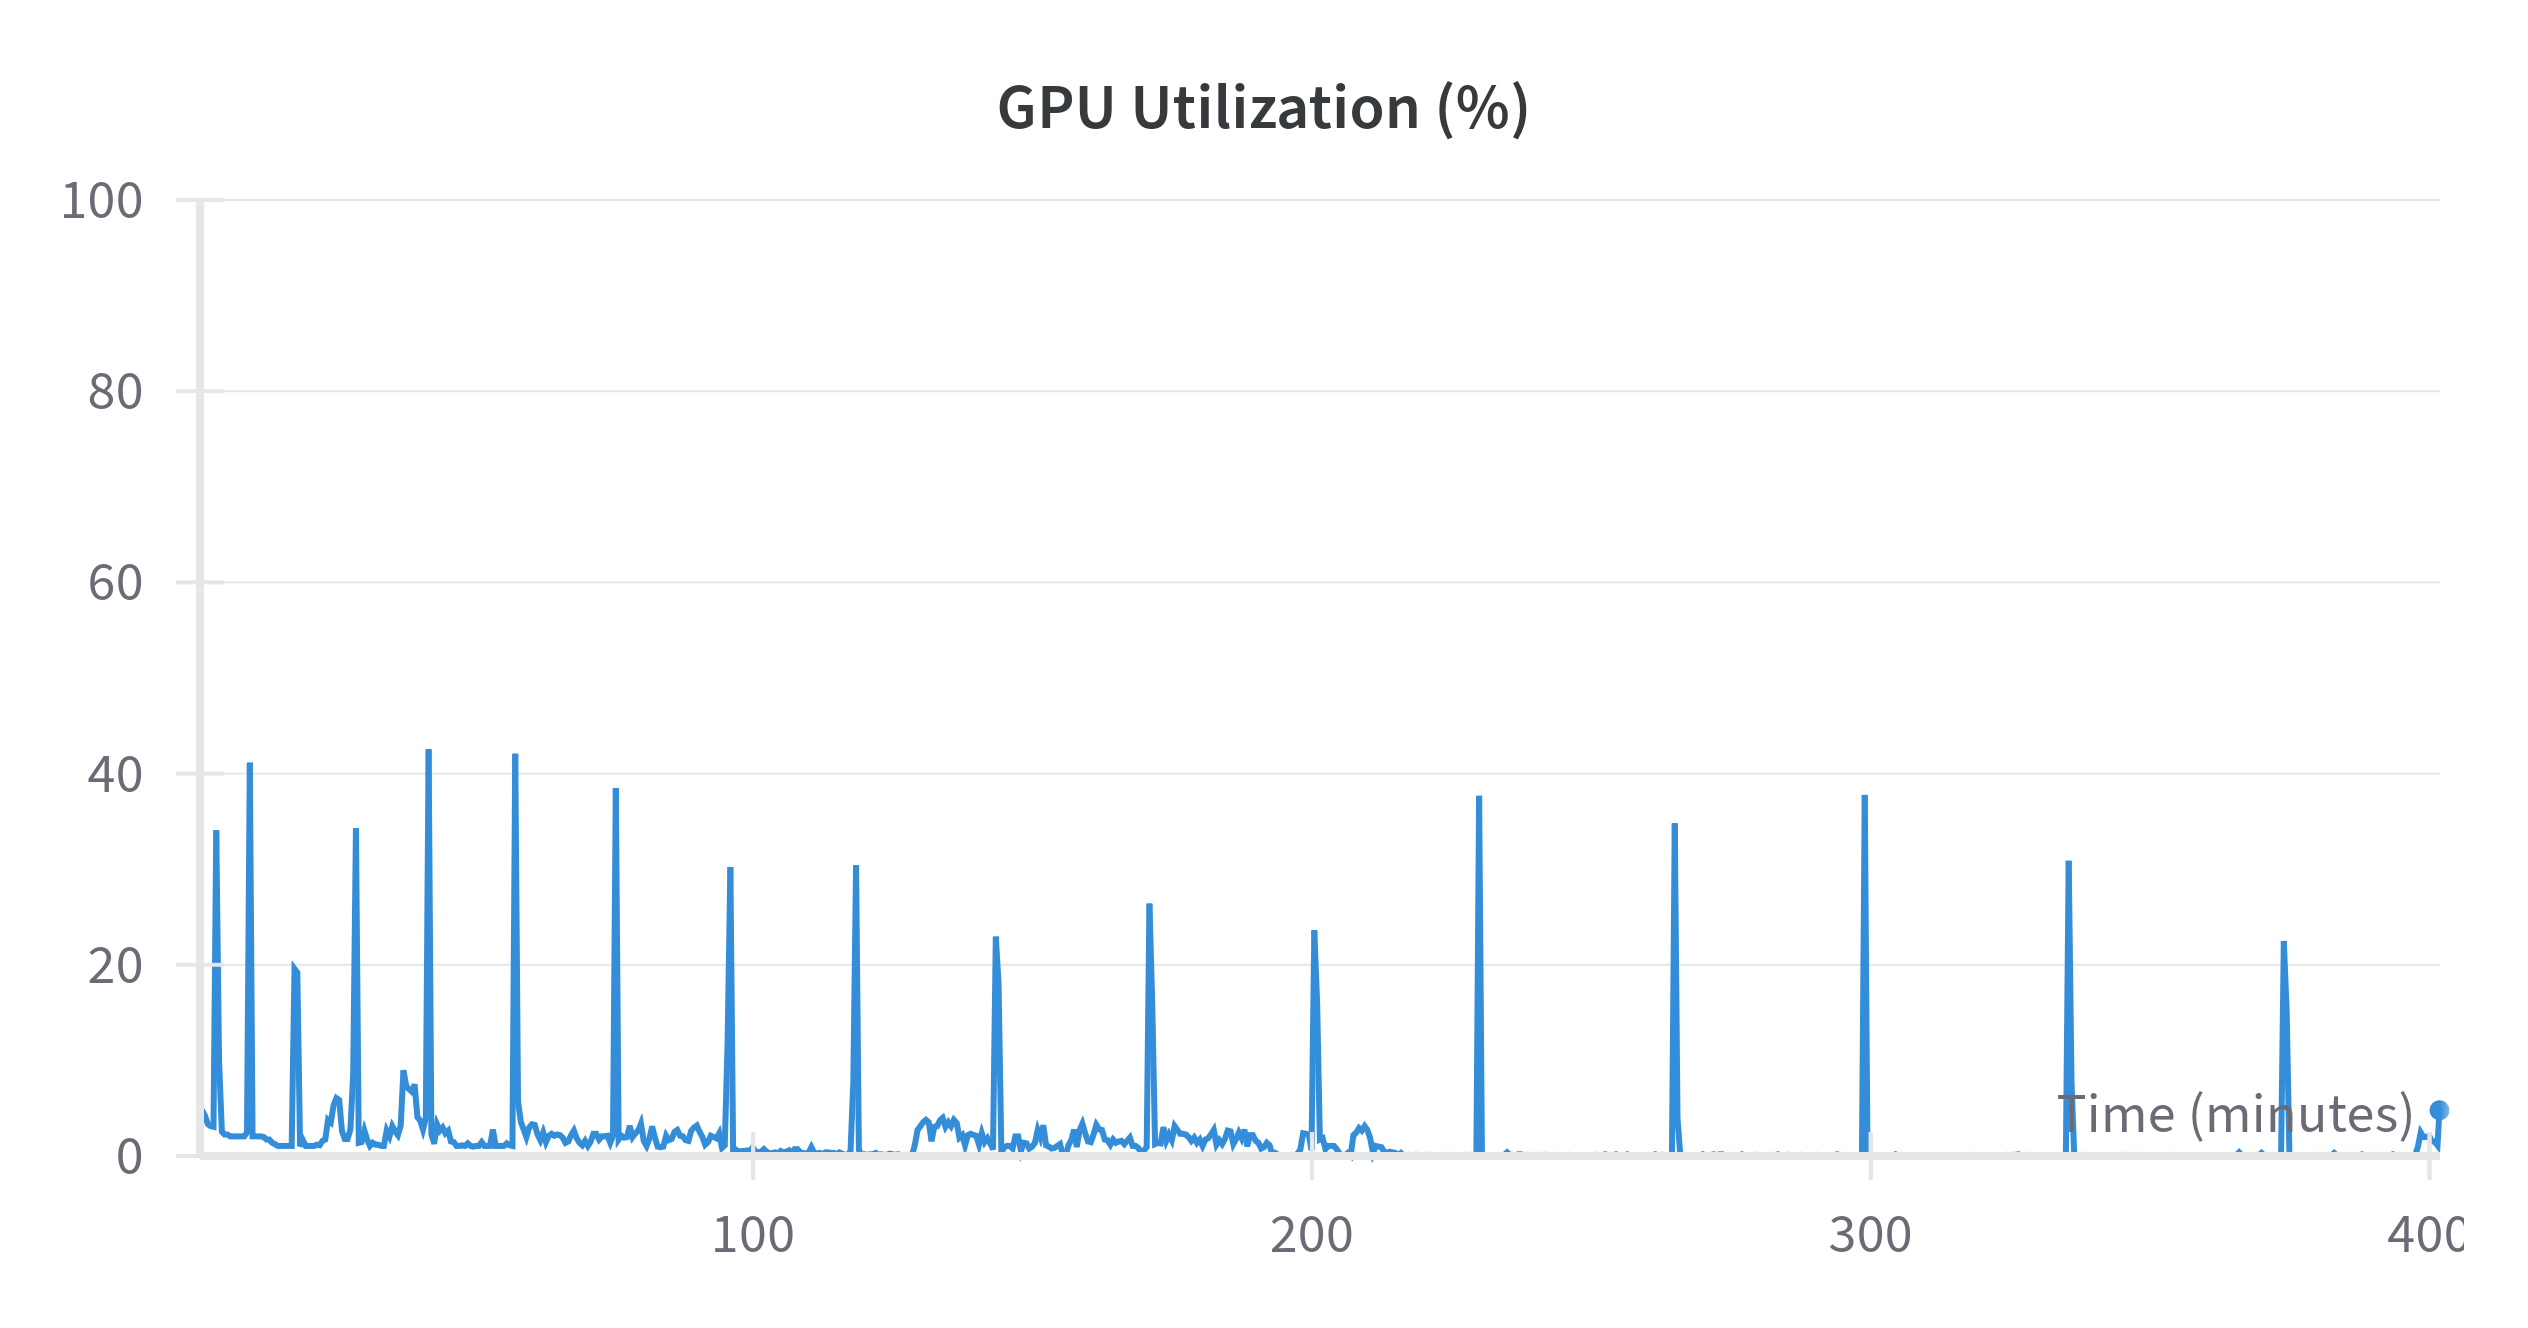
\includegraphics[width=0.8\textwidth]{figures/GPU_Utilization.png}
    \caption{GPU percentage usage while training an agent}
    \label{fig:gpu_memory_usage}
\end{figure}

\begin{figure}[H]
    \centering
    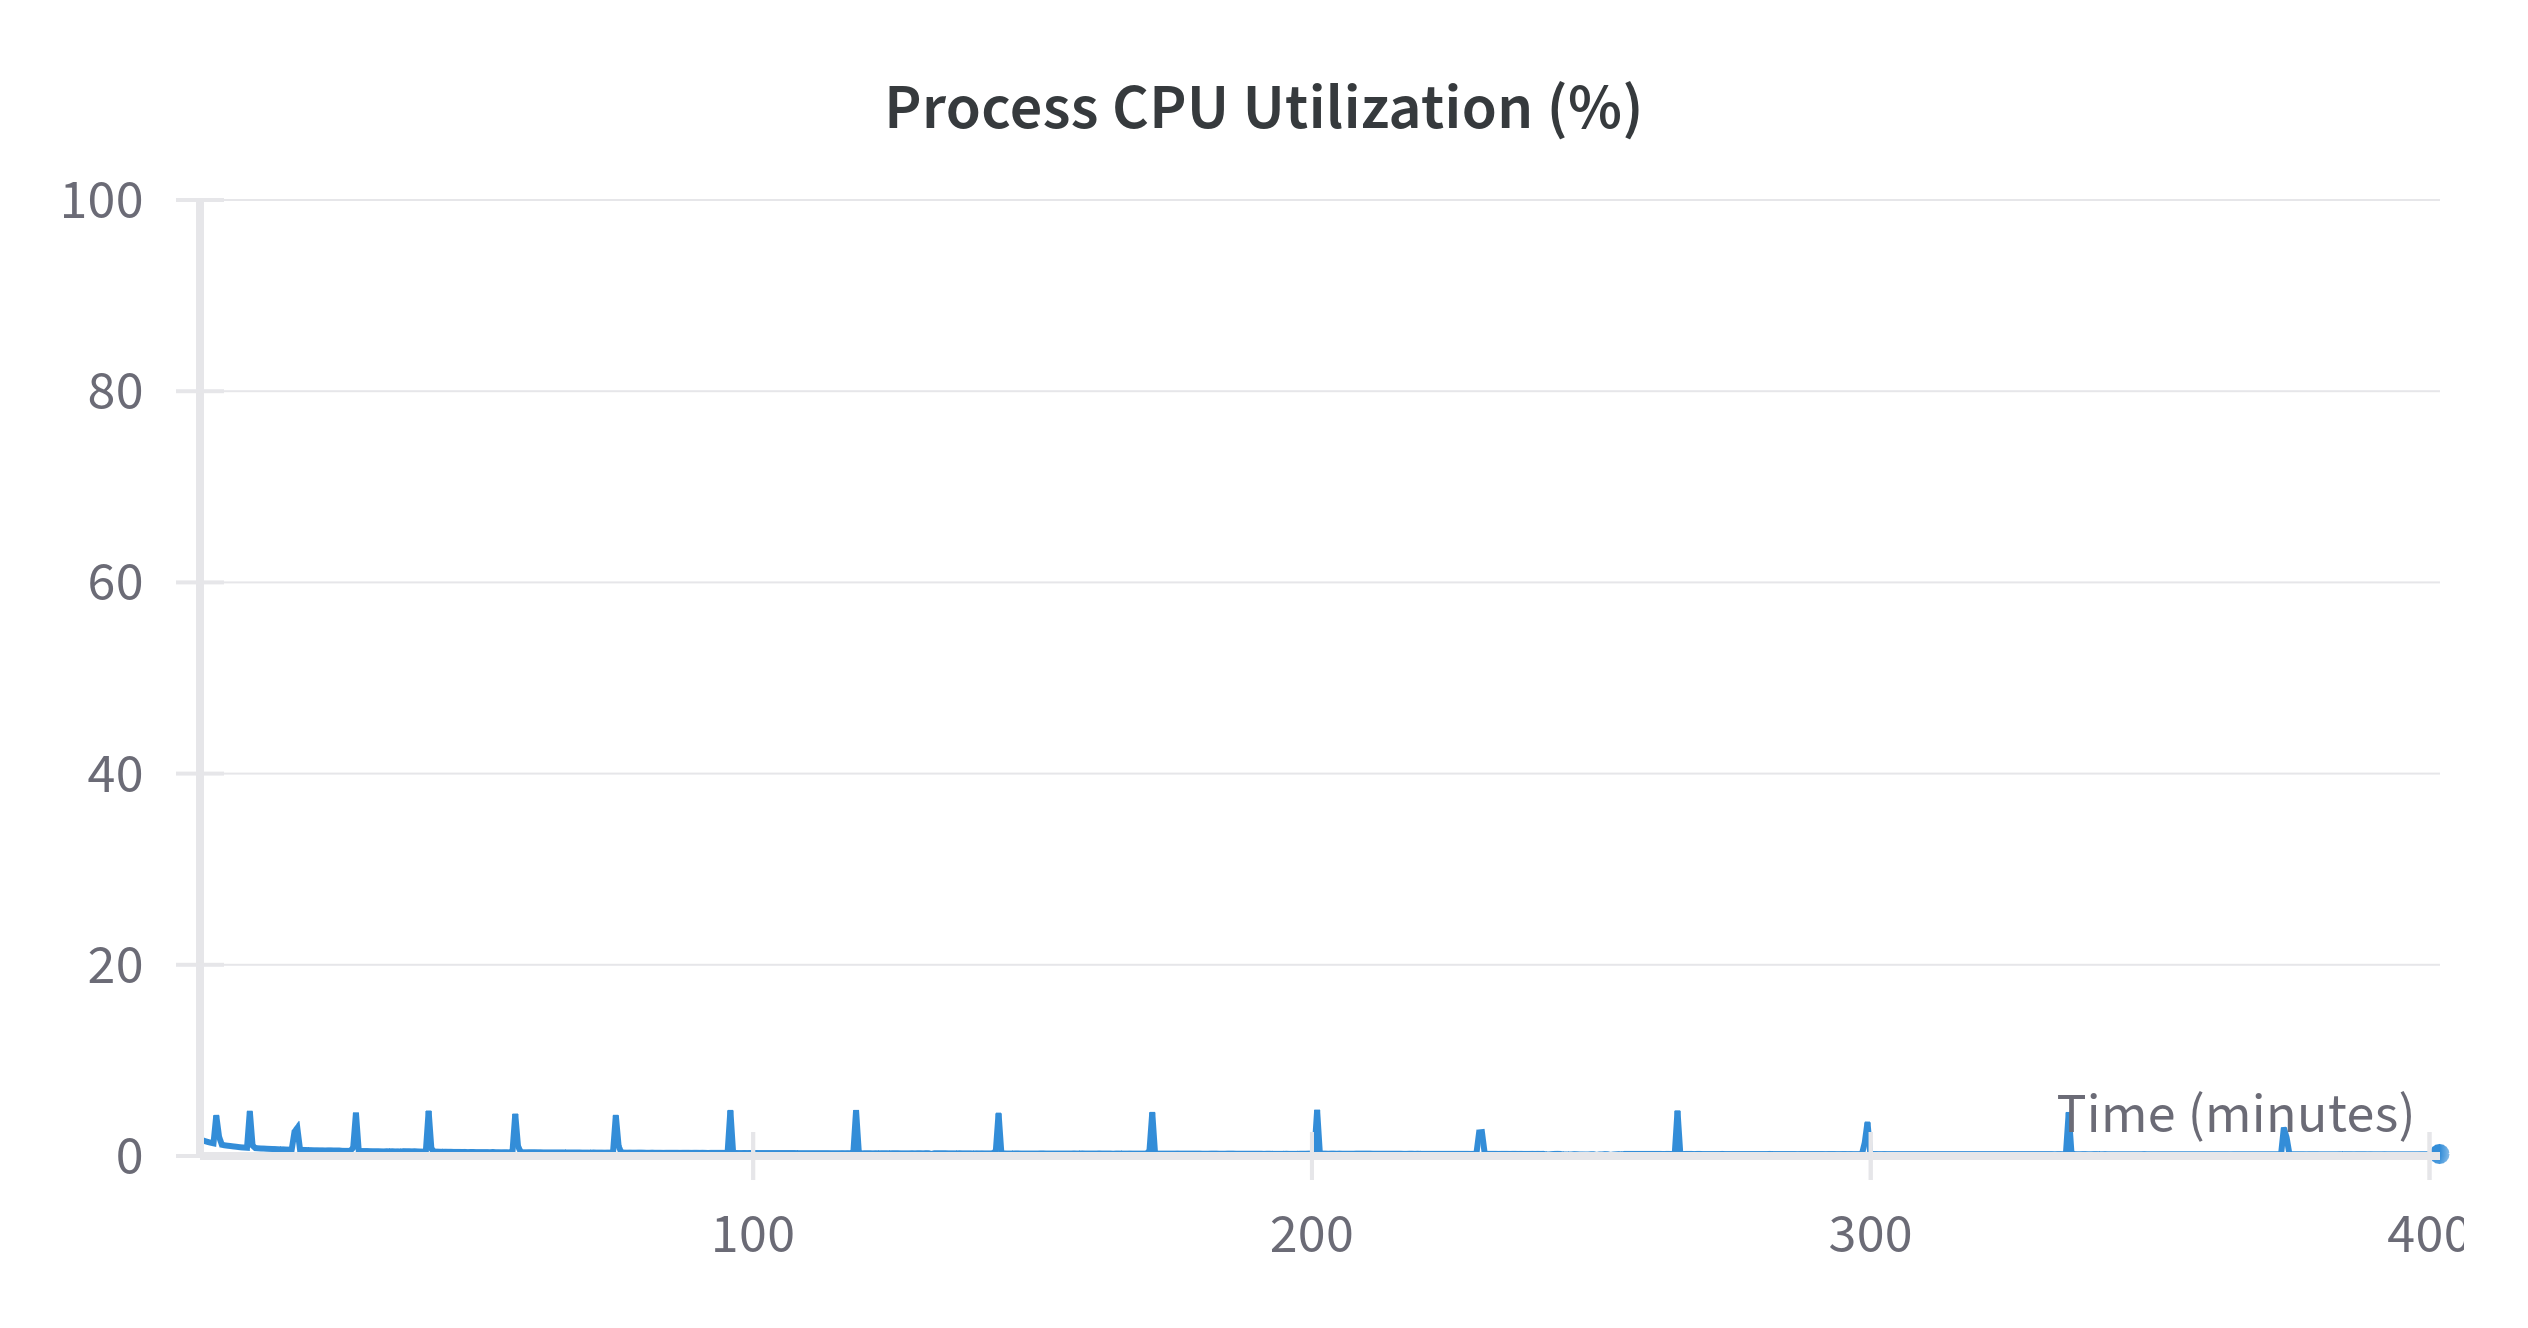
\includegraphics[width=0.8\textwidth]{figures/total_cpu_utilization.png}
    \caption{Total CPU usage while training an agent}
    \label{fig:ram_usage}
\end{figure}

\begin{figure}[H]
    \centering
    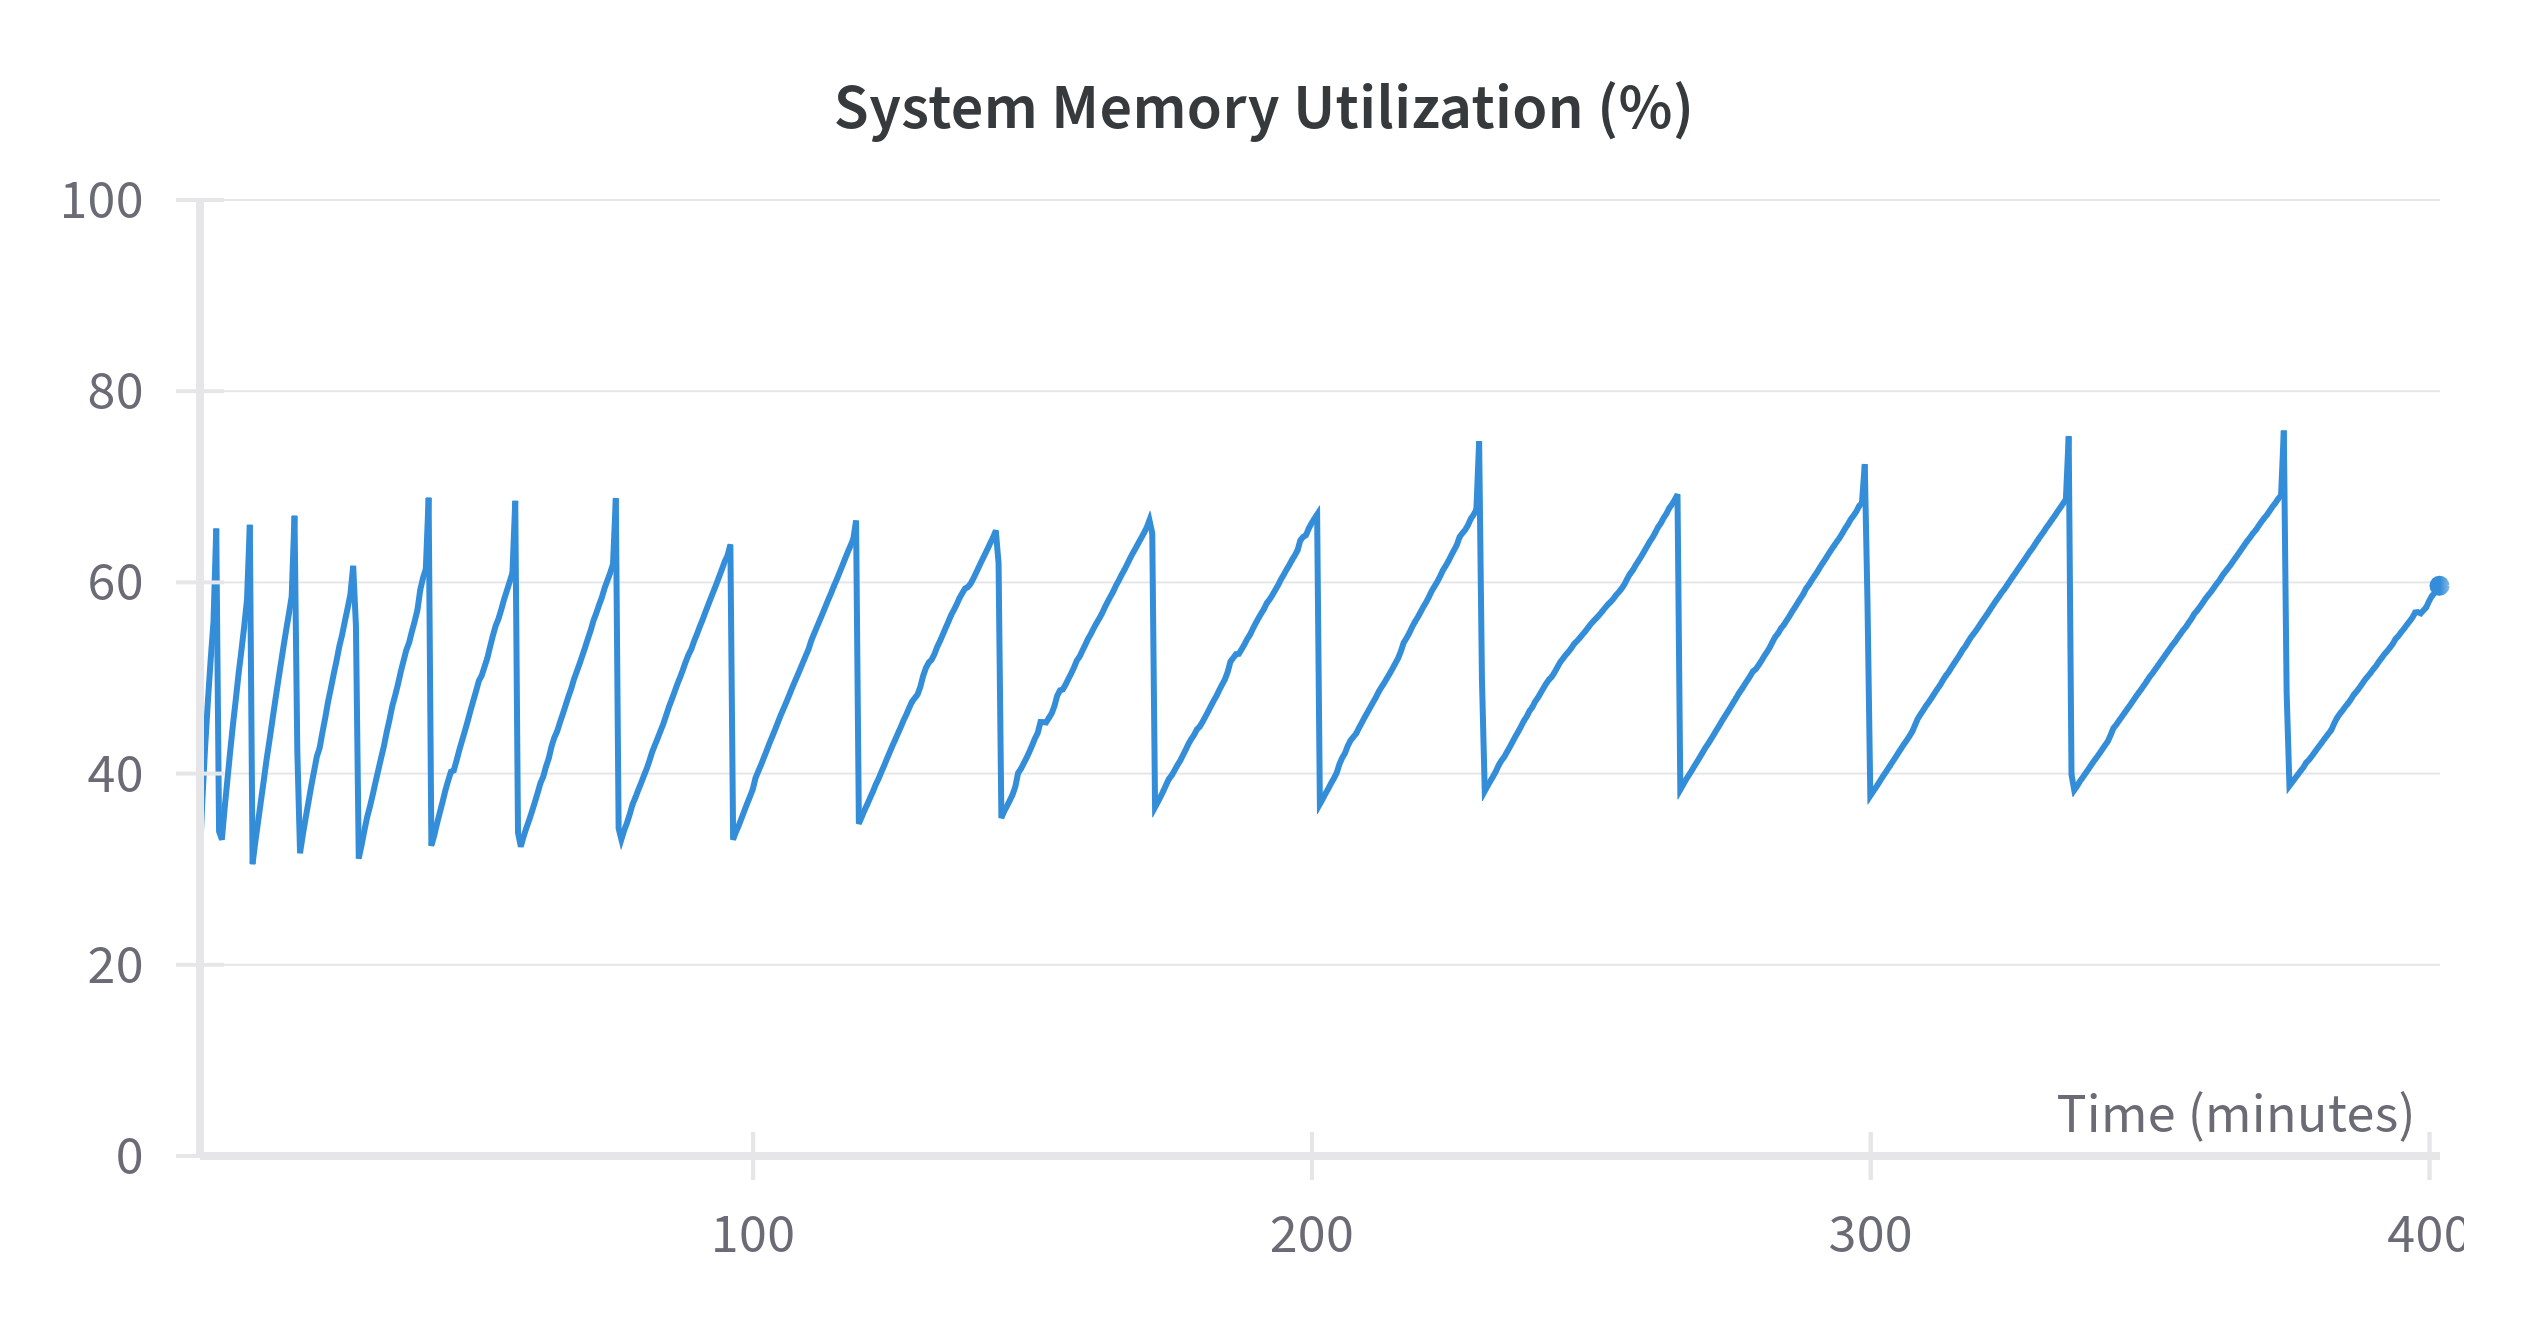
\includegraphics[width=0.8\textwidth]{figures/System_RAM_Utilization.png}
    \caption{Total RAM usage while training an agent}
    \label{fig:sys_memory_useage}
\end{figure}

From the three figures above, it can be seen that the GPU Utilization was low, with a maximum of 42.47\% peak usage. The CPU usage was also low, with a maximum of 4.71\% peak usage, while the Total RAM usage while training the agent was quite high, with a maximum of 75.82\% peak usage. The values provided in the figures above were taken from the wandb system monitor that was running while trianing the agents. In addition, these values have the possibility of being skewed, as the hardware running the training the agents was also running other system operating system essential processes. However, it is very evident that RAM was the bottleneck in training the agents.  

\subsection{Determining the optimal number of timesteps per episode}

Deciding on the total number of timesteps for each episode is a very difficult task to do as it is impossible to guage how many timesteps are needed for the agent to complete the first gym. The more timesteps per episode the more opportunities it has to explore the environment which would give it more potential options and paths it can take to find the optimal path with the given number of timesteps. However, the fewer timesteps per episode, the higher the risk that it is infeasible to complete the first gym and reward is maximized with the given number of timesteps, which would not include taking steps towards solving the problem of the environment. 

In addition, the fewer steps per episode, the more updates the policy will recieve. This is because the agent is trained for a specific number of timesteps instead of a number of episodes. Therefore, shorter episodes will lead to faster updates to the policy, which may lead to better policies and better data to train future instances. 

Due to the difficulty of determining the optimal number of steps per episode, the optimal number was determined by training numerous agents with different episode lengths and reward scaling. The objective of this research is to defeat the first gym leader, which is what the reward scale and episode length was tuned to complete. In the end, the number of steps per episode was decided to be 1,500. 

The wandb workspace with evidence and data of the training of the agents can be found at the following link: \url{https://wandb.ai/liam3323/pokemon-red-train}

\subsection{Data Recording}

Collecting data and graphing the results of the policy during training was straight forward. The wandb integration with stablebaselines3 meant that the data was automatically sent to the wandb server and graphed as it progressed for each timestep. This was very benefical during training of the agent as it allowed for agent's growth and change over time be monitored.  

\section{Evaluation}

Having explained the details of the environment and the algorithms used, this section will go into detail about the details of the configuration of the experiments and the results of the experiments. The details of the training configuration for each algorithm and the reason for these decisions will be discussed. For each algorithm compared, the best perfoming agent will be determined and chosen to be used as the agent to be compared to the other best performing agents. When deciding the best performing agent, multiple factors will be considered such as the total reward, loss, amount of exploration and amount of battling. The results of the experiments will be discussed, compared to each other and evaluated to determine how well they were able to balance out both battling and navigation.

\subsection{Training Configuration}

The training configuration for each algorithm was set to be the same for each algorithm. Each agent was trained for a total of 40 million steps and a gamma rate of 0.998 within the environment with a batch size of 64. Each algorithm used the default hyperparameters implemented within the stablebaselines3 library and each agent was trained with the exact same representation of the environment with no changes to the reward scaling and reward functions. 

\subsubsection{Hyperparameter Tuning}

It was mentioned previously that each algorithm would be hyperparameter tuned so that they were compared fairly. However, the hyperparameters were not tuned for each algorithm because of the amount of time it would take to tune each hyperparameter for each algorithm. It would take 5-7 hours to train a single agent, which would mean that it would take countless more for each hyperparameter for each algorithm to be tuned. Therefore, the default hyperparameters implemented by stablebaselines3 were used for each algorithm to ensure that the agents were compared fairly \cite{stablebaselines3}.

\subsection{DQN}

The training script used to train all 4 agents can be found within the research paper's GitHub repository under ``run\_baseline\_DQN.py''. A total of 10 parallel instances of the environment was trained at the same time to train for 2,667 episodes total, where each episode is 1,500 steps long. This totals up to 40,00,500 steps in total. The performance of the 4 agents can be seen on figure \ref{fig:agent_eval_all_dqn}. 

\begin{figure}[H]
    \centering
    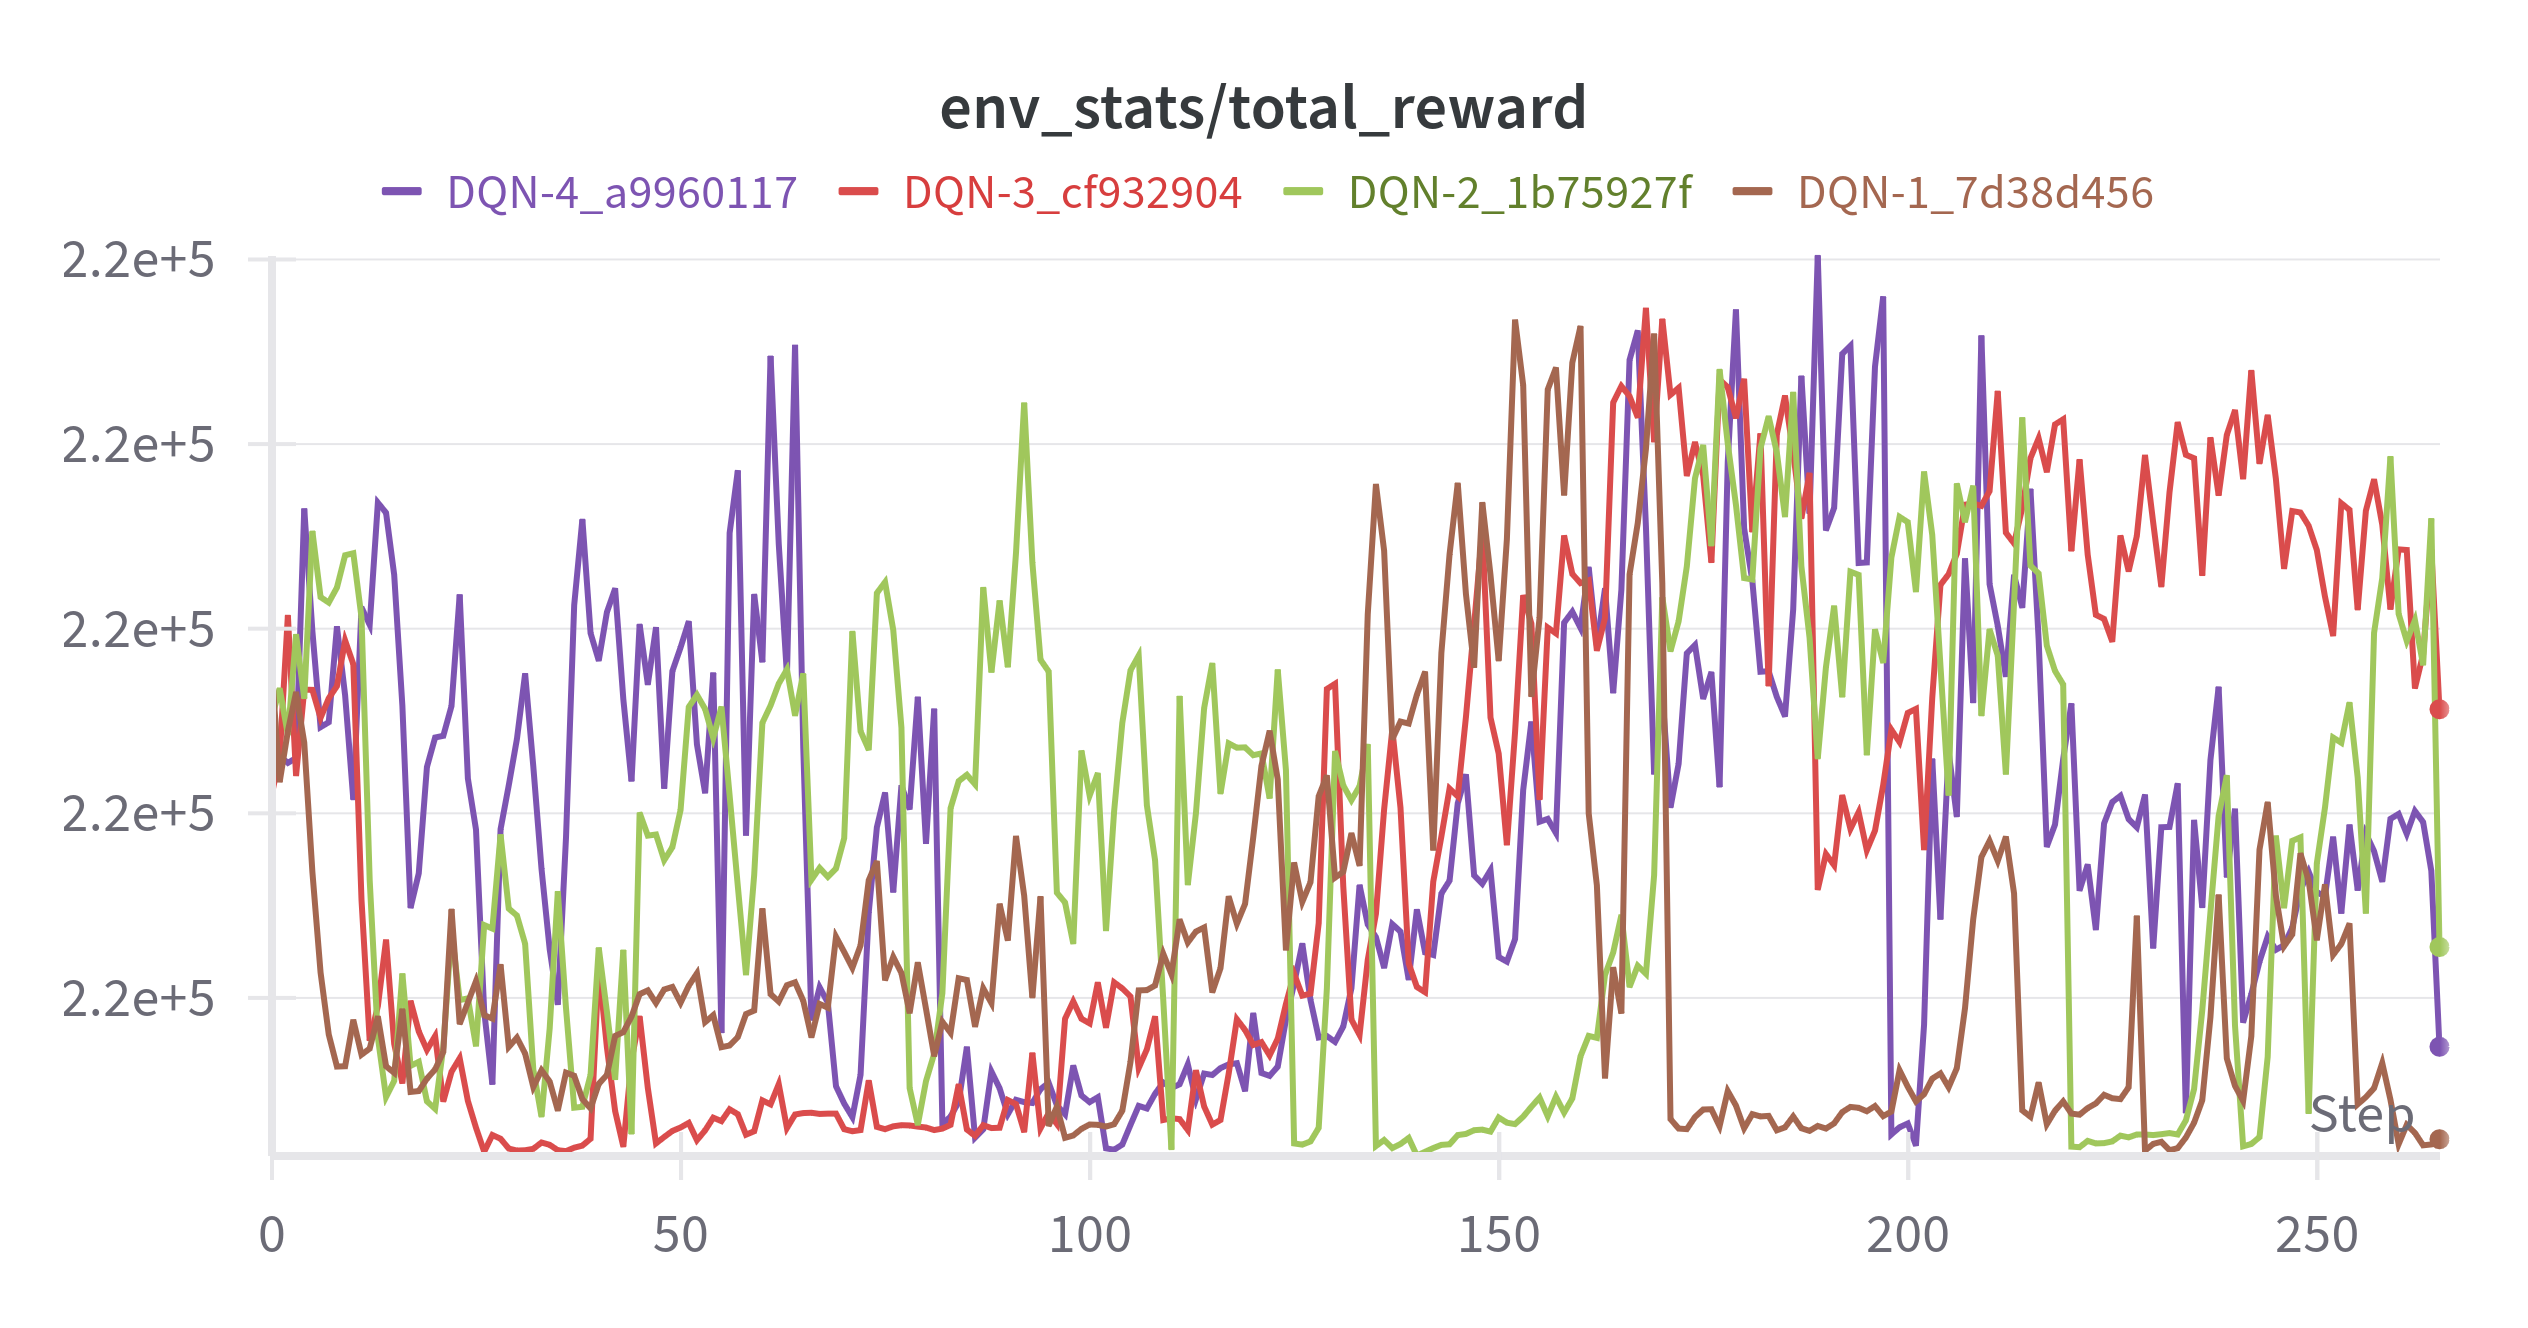
\includegraphics[width=0.8\textwidth]{figures/DQN_TotalReward.png}
    \caption{Total Reward of All DQN Agents}
    \label{fig:agent_eval_all_dqn}
\end{figure}

Figure \ref{fig:agent_eval_all_dqn} shows the performance of all 4 DQN agents of total\_reward against episode. The figure shows all 4 performing agents did not show signs of reaching the optimal policy as the total reward did not reach a plateau nor did the total reward show a dramatic difference from the start of training to the end of training. Moreover, the graph displays the average total reward of 10 episodes, which is why the x-axis is not in steps or go up till the 2,667 episodes that the agents were trained for.

\begin{figure}[H]
    \centering
    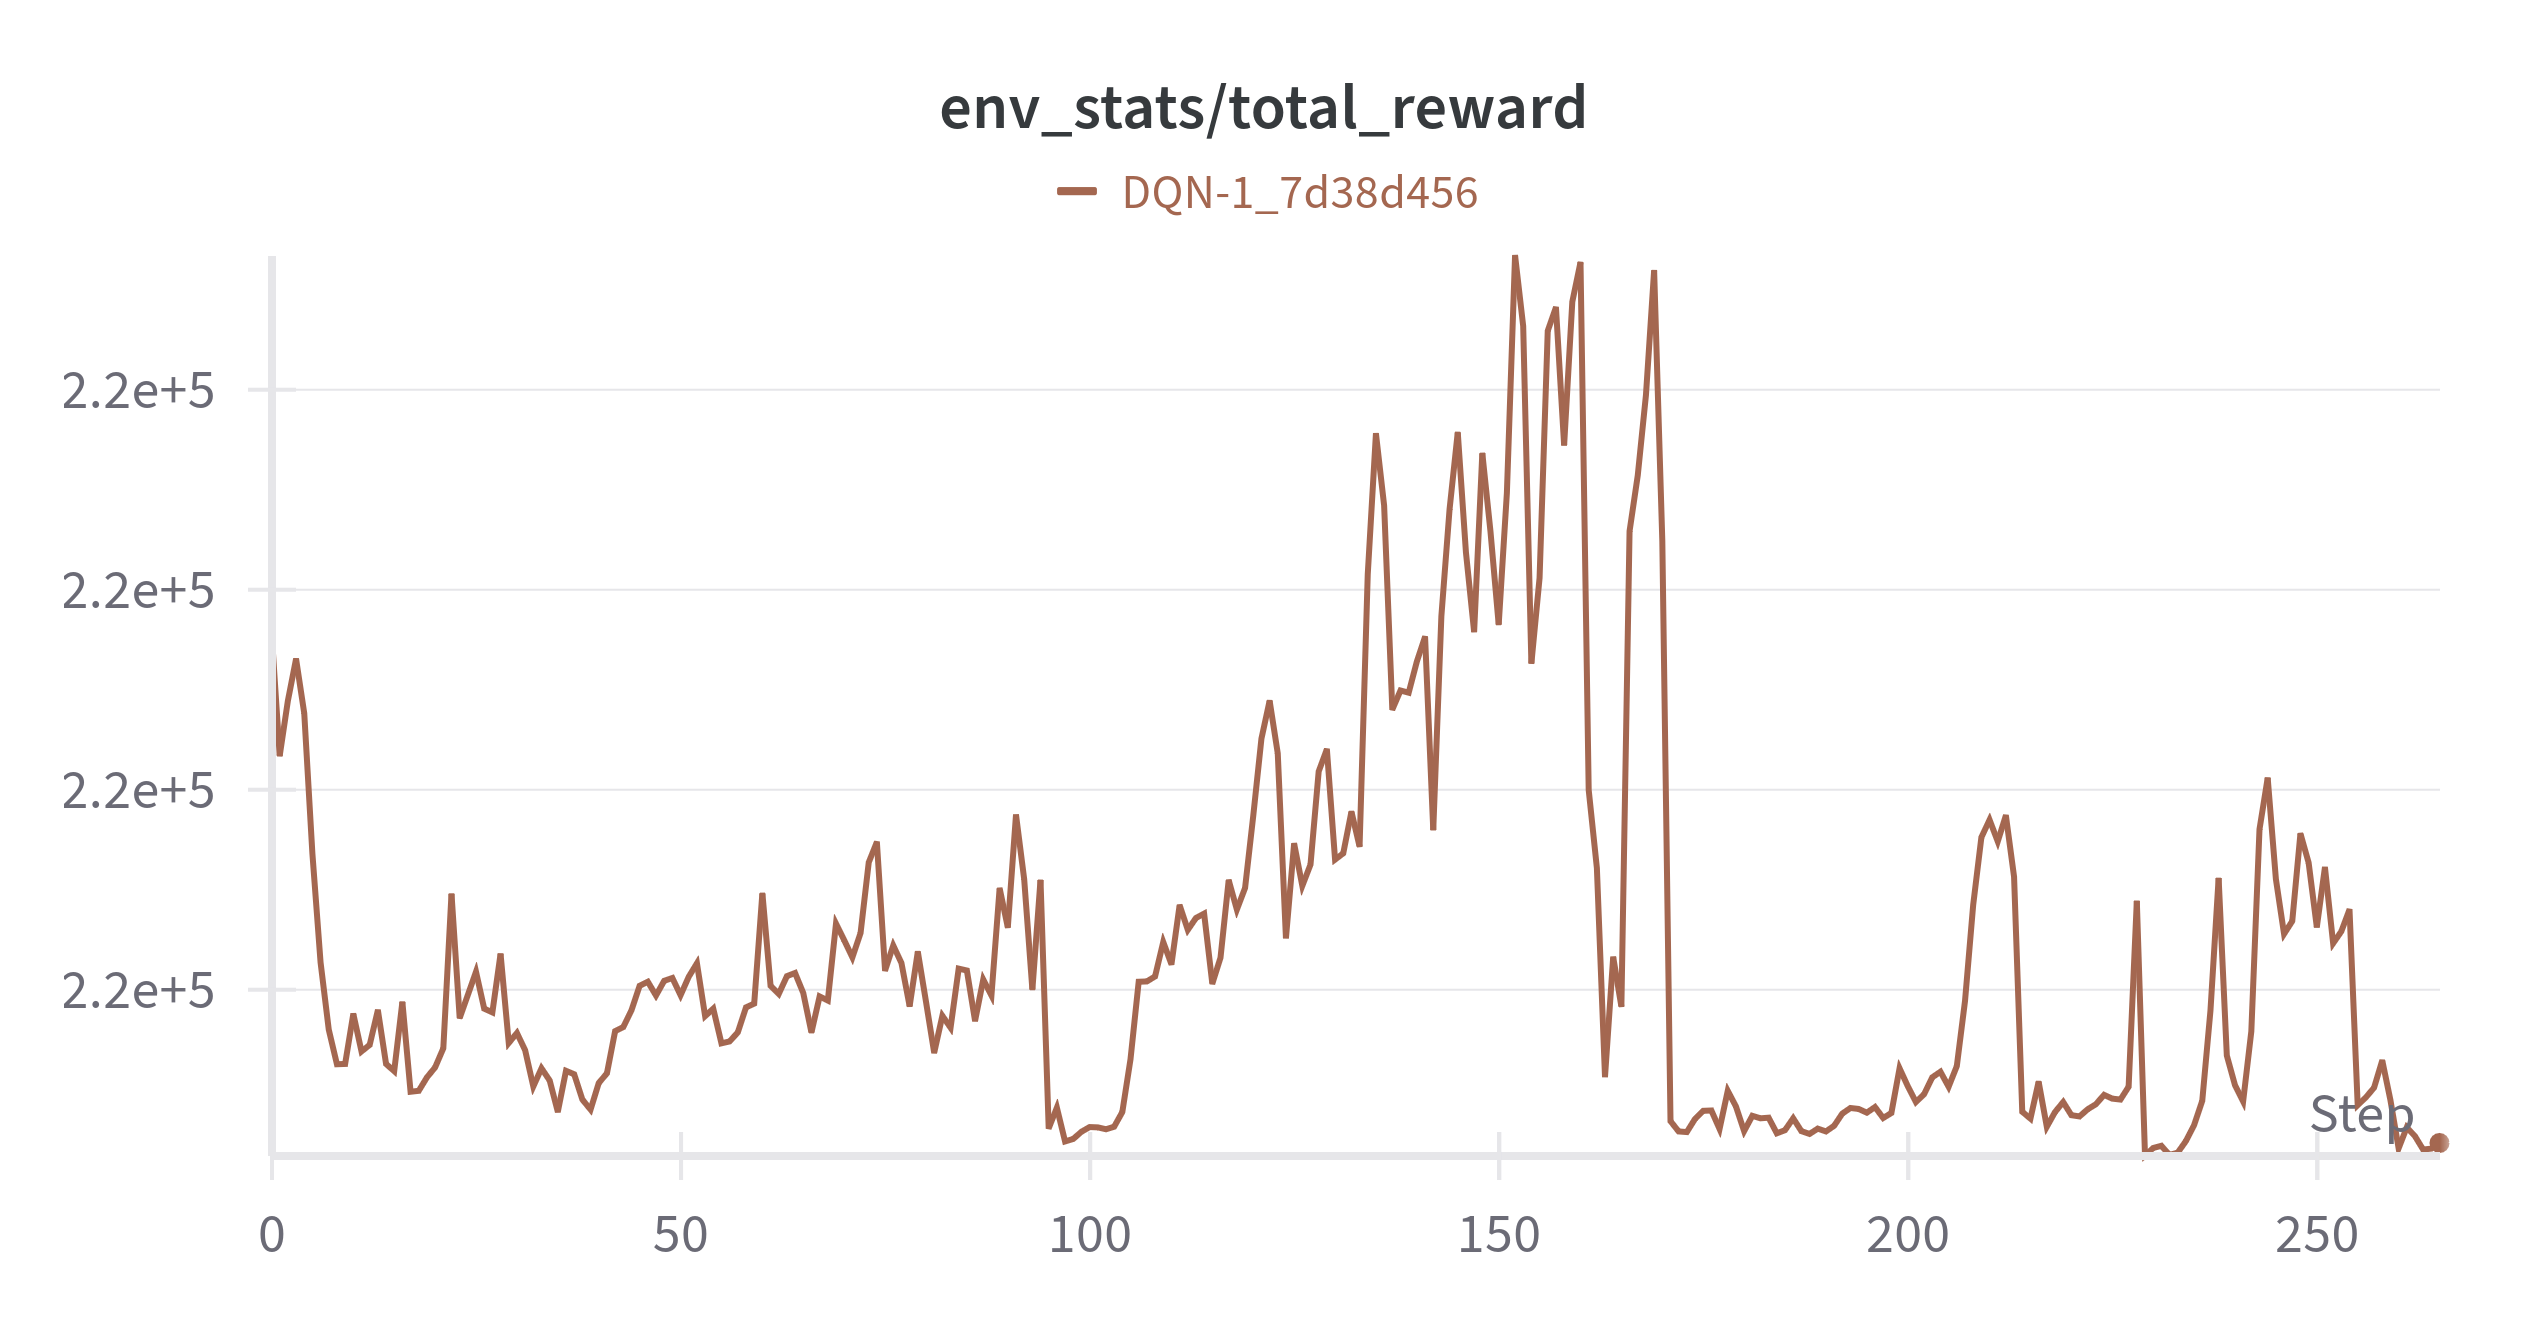
\includegraphics[width=0.7\textwidth]{figures/DQN-1_TotalReward.png}
    \caption{Total Reward of DQN Agent 1}
    \label{fig:agent_eval_dqn_1}
\end{figure}

Figure \ref{fig:agent_eval_dqn_1} shows the performance of the first DQN agent of total\_reward against episode. The figure shows that the agent did not show signs of reaching the optimal policy as the performance of the agent peaked at around 150 episodes followed by a sharp fall in performance. This suggests that the agent was still exploring the environment and was not ready to start exploiting the environment using its already known information, as the sharp fall in performance was below the starting performance of the agent.

\begin{figure}[H]
    \centering
    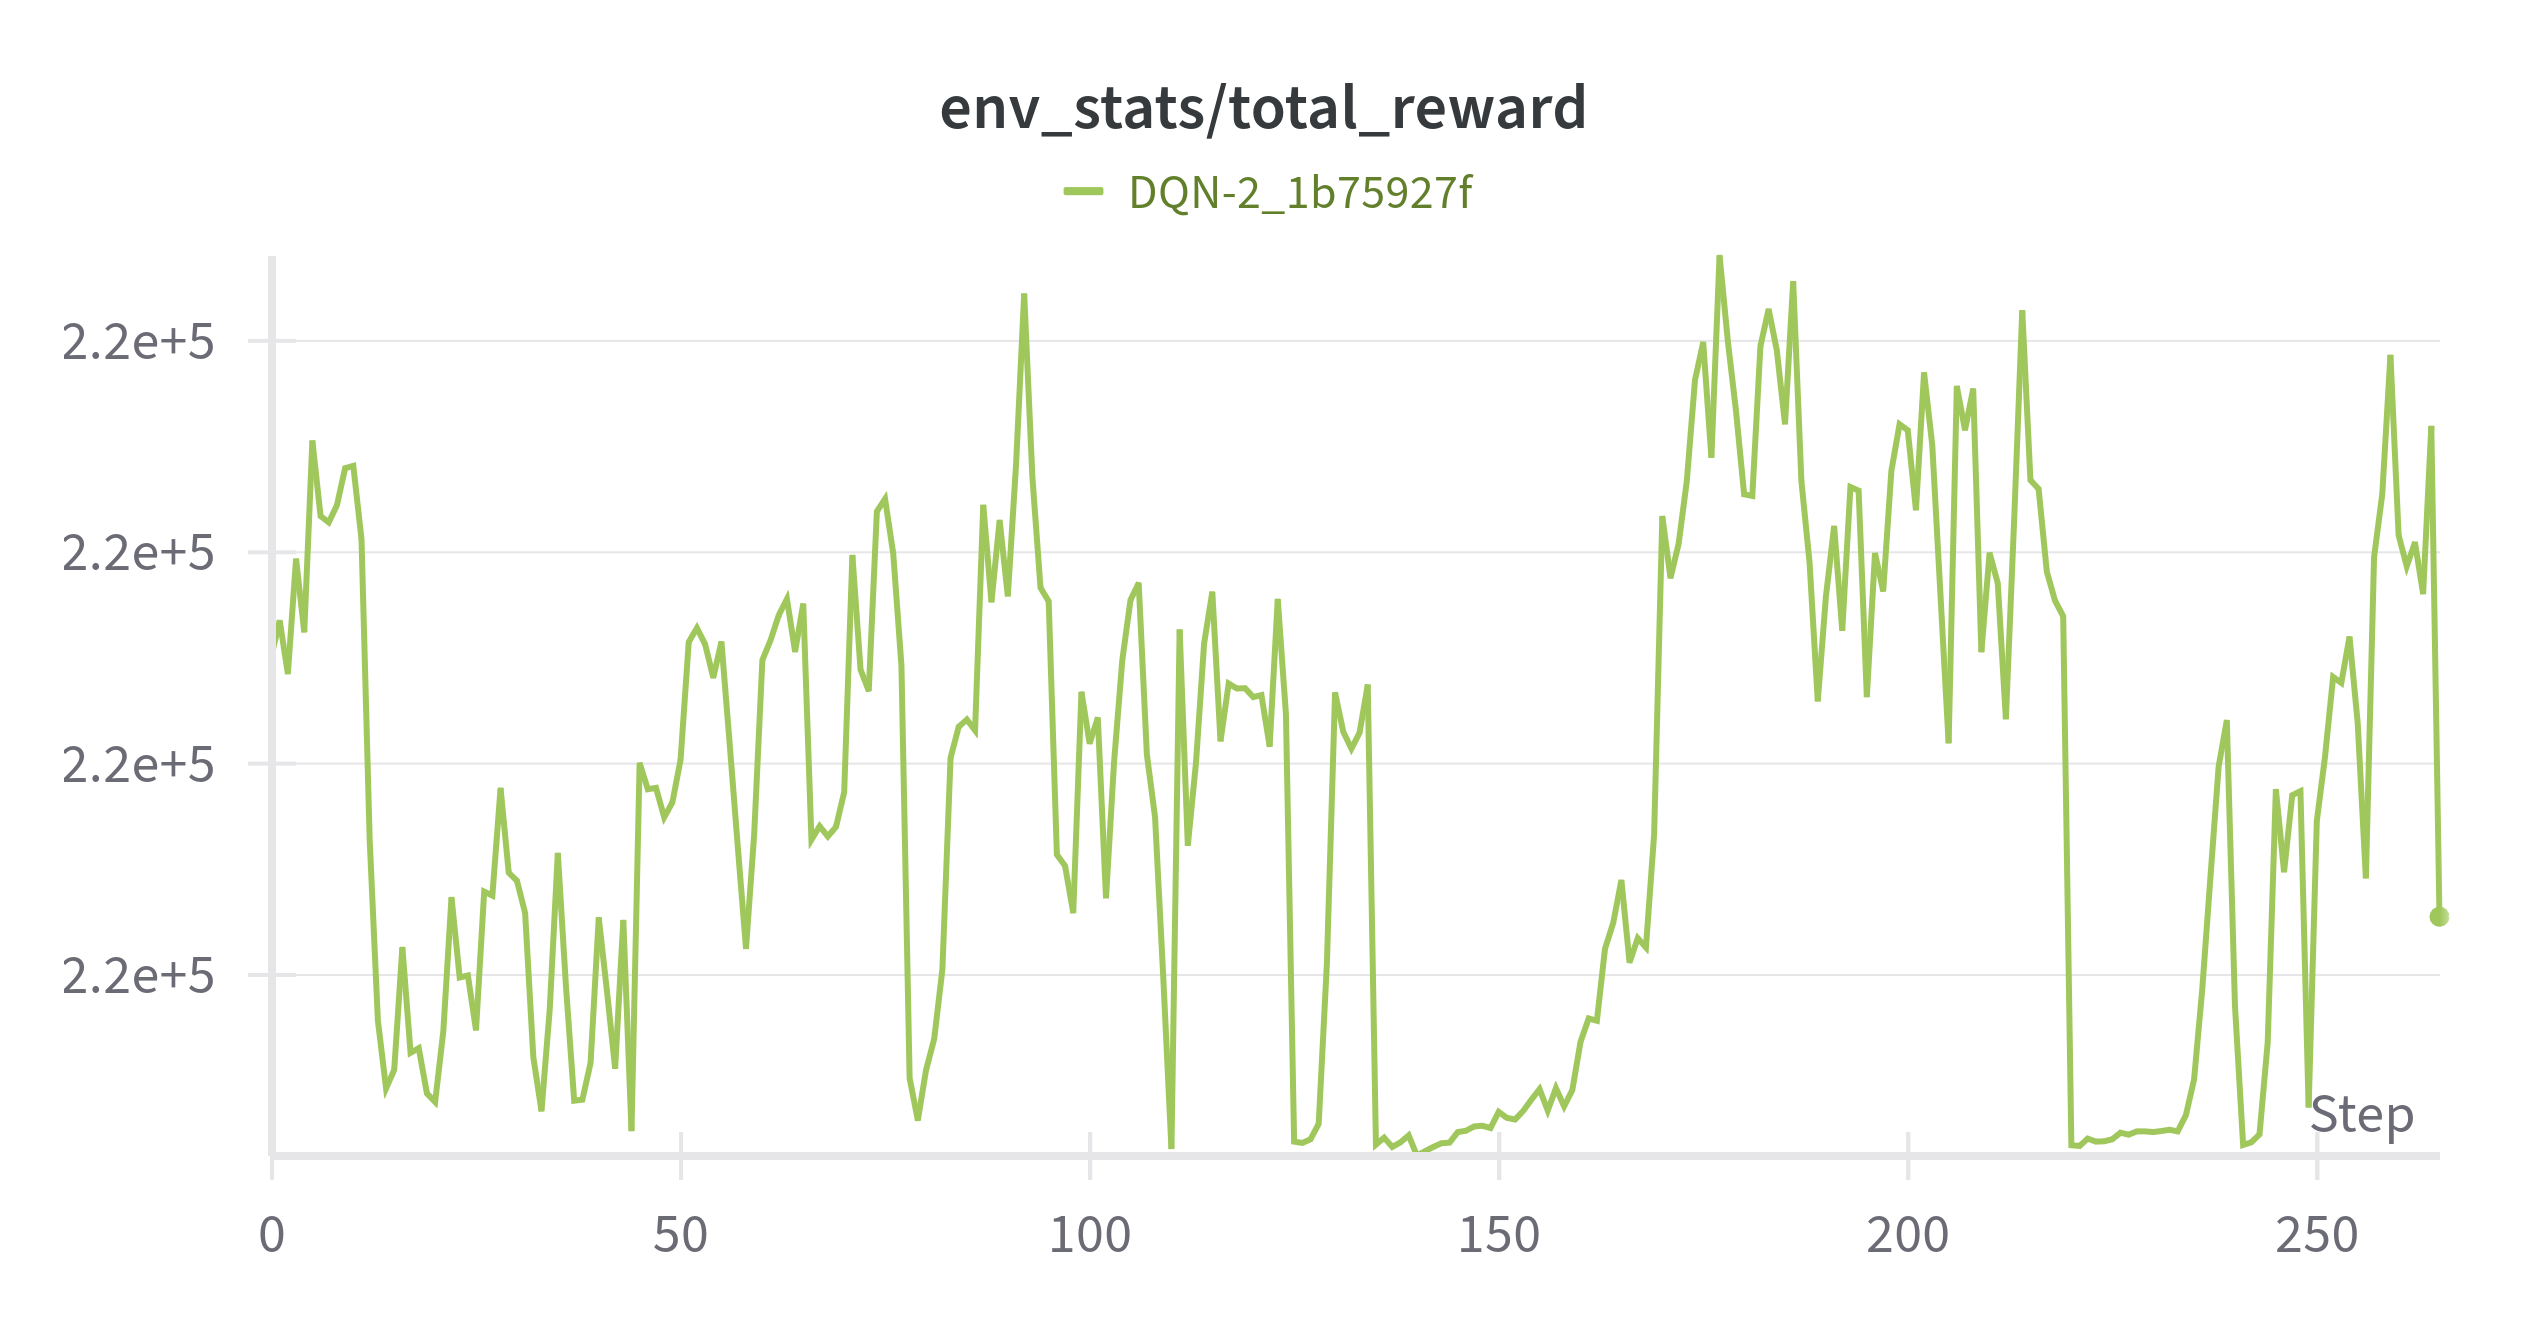
\includegraphics[width=0.7\textwidth]{figures/DQN-2_TotalReward.png}
    \caption{Total Reward of DQN Agent 2}
    \label{fig:agent_eval_dqn_2}
\end{figure}

Figure \ref{fig:agent_eval_dqn_2} shows the performance of the second DQN agent of total\_reward against episode. The figure shows that the agent did show signs of significant amount of exploration, as there was a range of episodes where the agent had high and low performance. This suggests that the agent was still exploring the environment. However, the agent did have a consistently high amount of performance between episodes 170 and 210.

\begin{figure}[H]
    \centering
    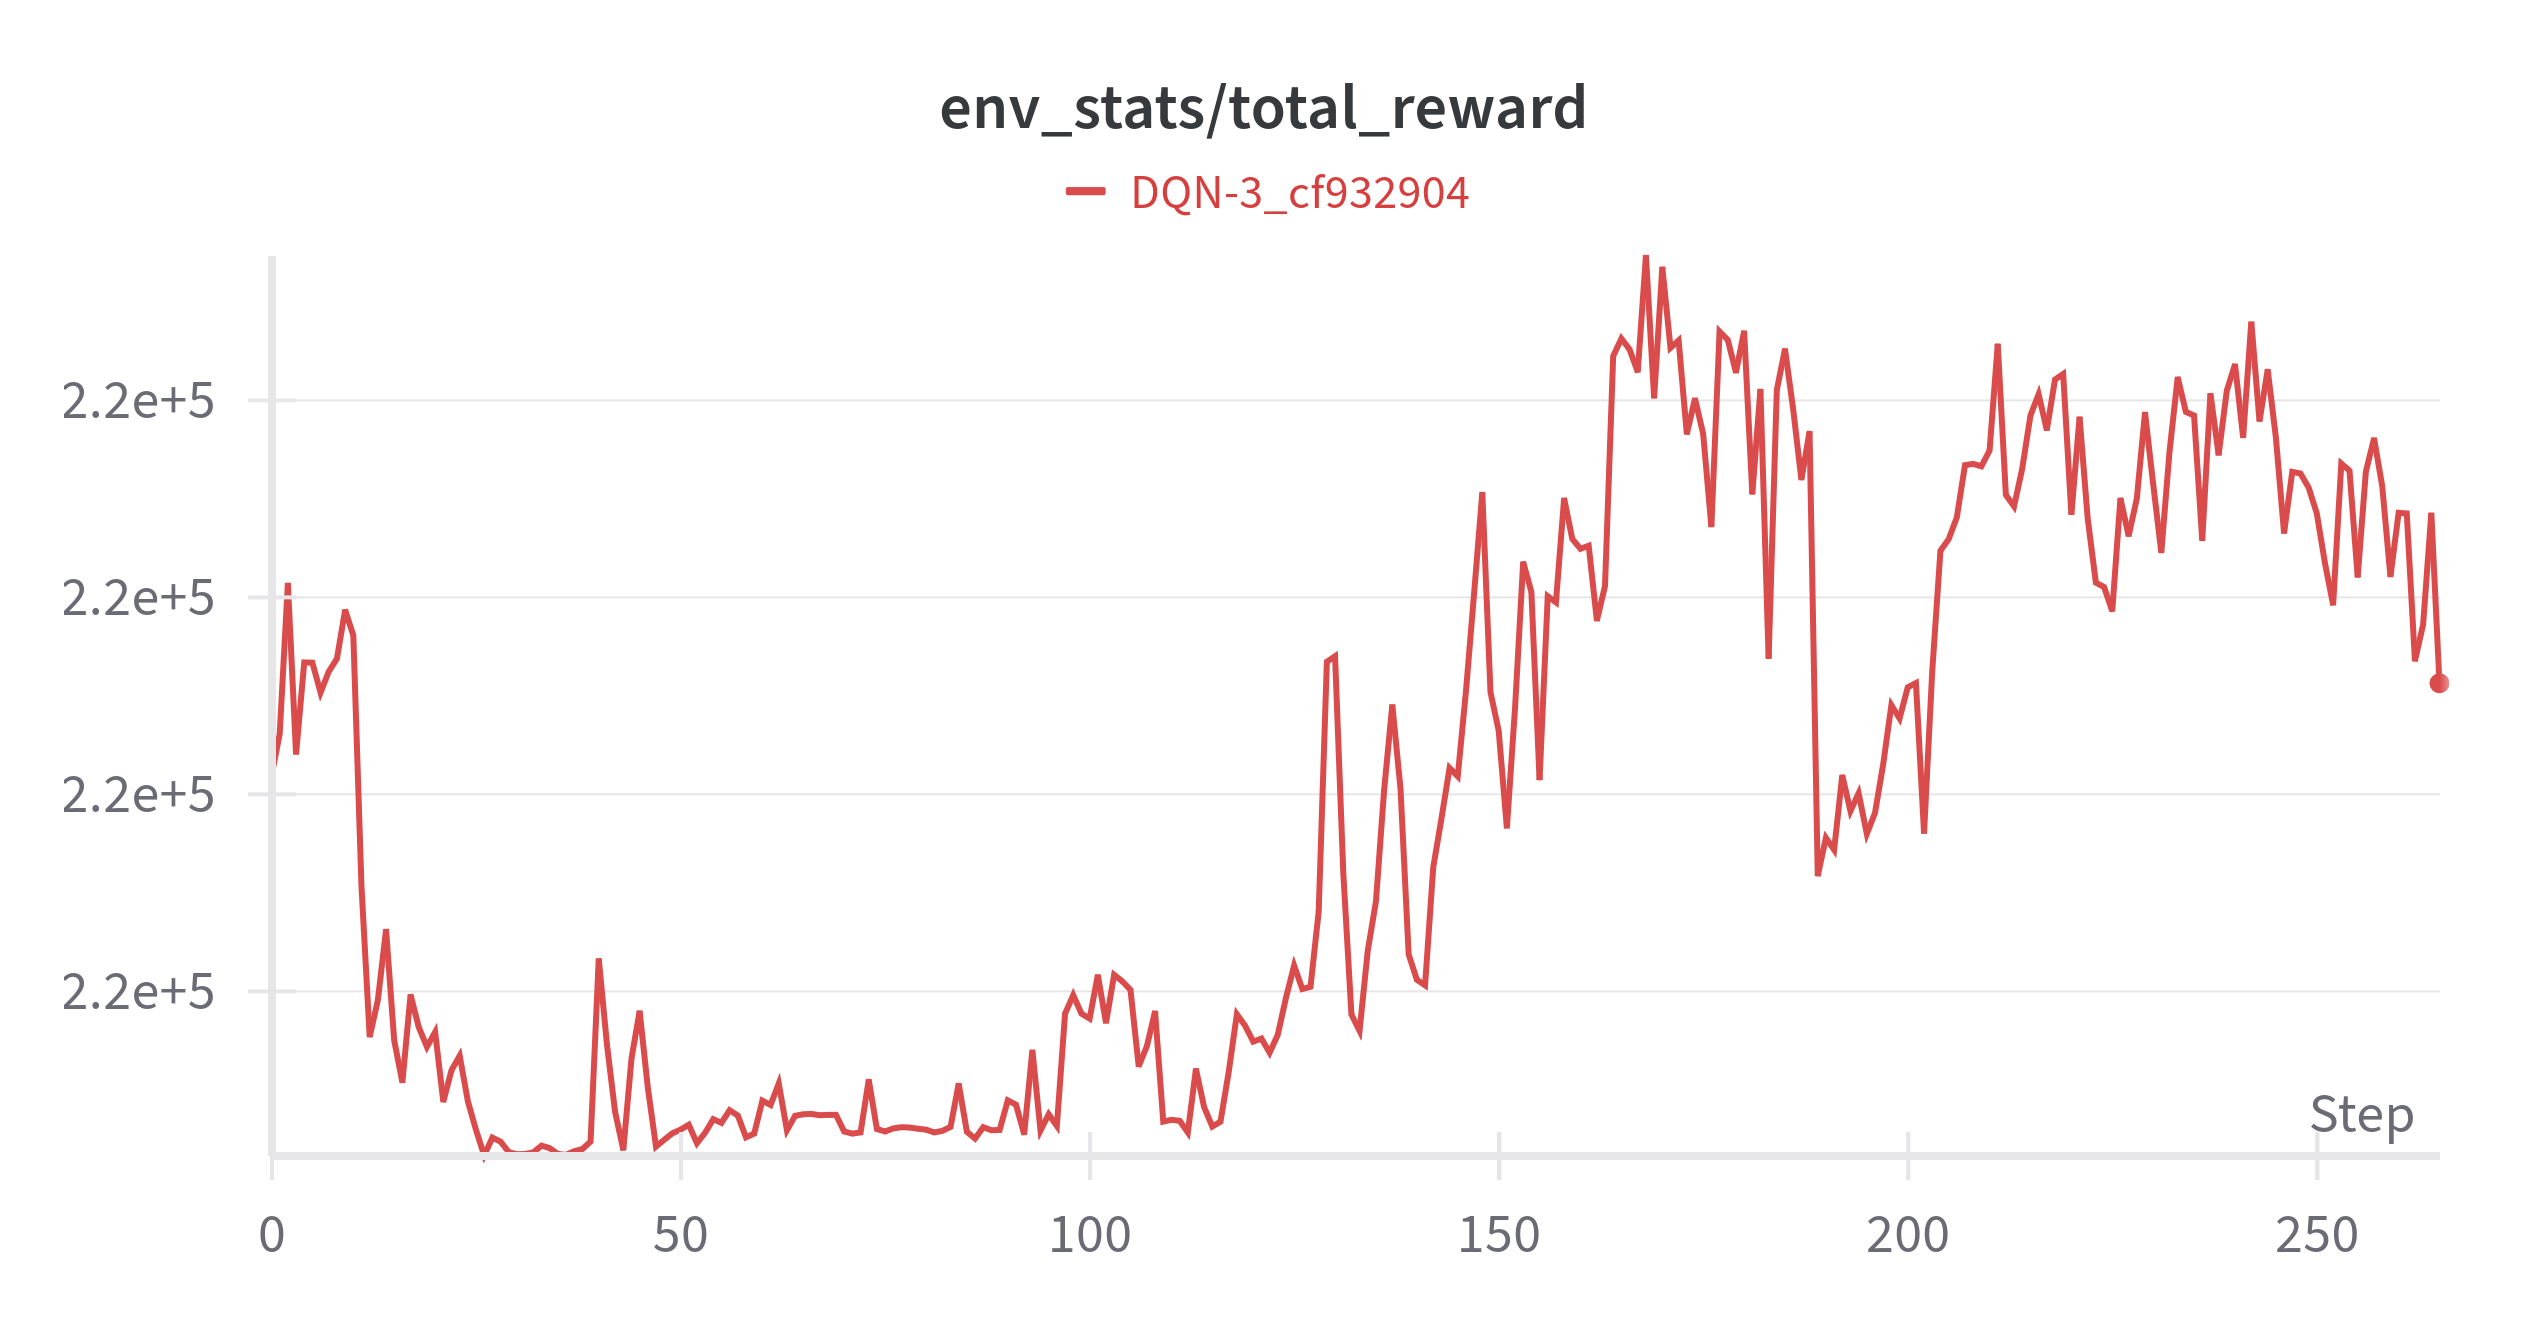
\includegraphics[width=0.7\textwidth]{figures/DQN-3_TotalReward.png}
    \caption{Total Reward of DQN Agent 3}
    \label{fig:agent_eval_dqn_3}
\end{figure}

Figure \ref{fig:agent_eval_dqn_3} shows the performance of the third DQN agent of total\_reward against episode. The figure shows that the agent did show signs of exploration, as the training of the agent started with a low amount of performance and gradually increased in performance between episode 10 and 150. This suggests that the agent was able to slowly learn the environment that was trained on and shows signs of gradual learning. Moreover, the agent was able to reach a peak performance at around episode 150 and is the best performing agent out of the DQN agents so far due to its consistently high performance. 

\begin{figure}[H]
    \centering
    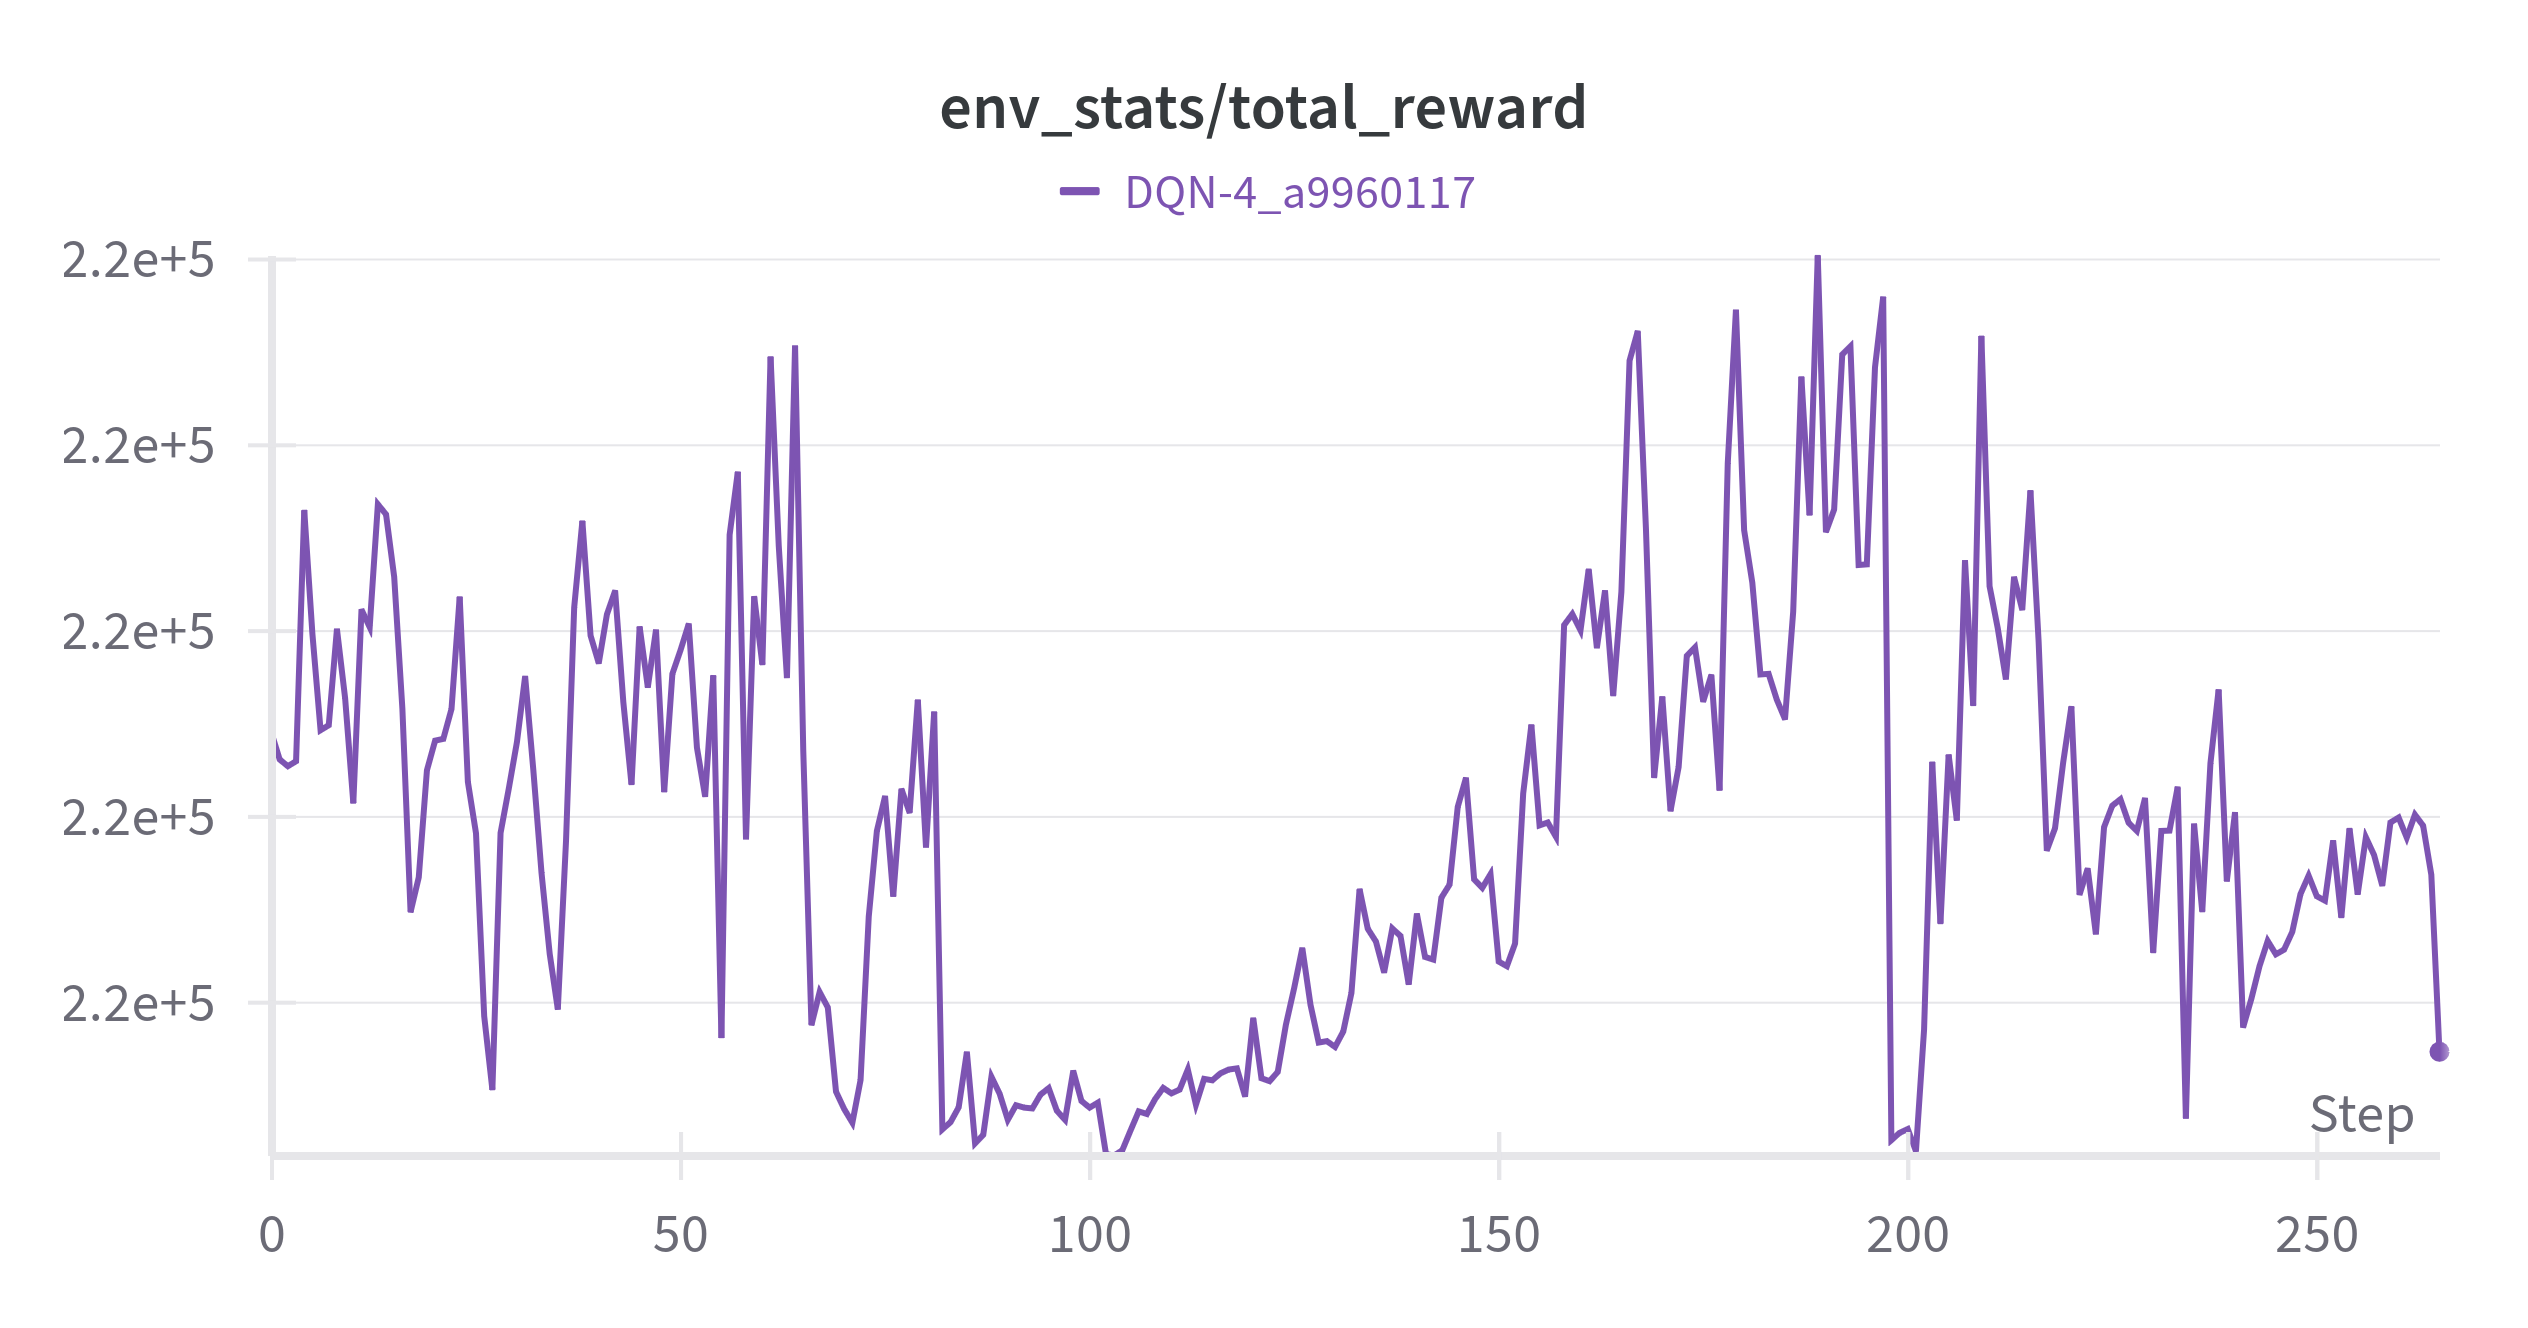
\includegraphics[width=0.7\textwidth]{figures/DQN-4_TotalReward.png}
    \caption{Total Reward of DQN Agent 4}
    \label{fig:agent_eval_dqn_4}
\end{figure}

Figure \ref{fig:agent_eval_dqn_4} shows the performance of the fourth DQN agent of total\_reward against episode. The figure shows that the agent shows weak signs of an understanding of the environment due to its low performance throughout the training. The agent did not show any signs of consistently high performance as drops in performance always followed high peaks. This highly suggests that the agent was still exploring the environment and never reached a point where it was able to exploit the environment using its already known information.

In conclusion, the best performing DQN agent from the list of 4 agents is agent 3 because of its consistently high performance throughout the training. The agent was able to learn the environment and exploit the environment using its already known information, which is evident from the inital low amount of reward followed by a strong growth in average reward. This further suggests that the agent shows signs of being able to go through cycles of learning and exploiting before reaching the optimal policy. 

\subsection{QR-DQN}

The training script used to train all 4 agents can be found within the research paper's GitHub repository under ``run\_baseline\_QRDQN.py''. A total of 8 parallel instances of the environment was trained at the same time to train for 3,333 episodes total, where each episode is 1,500 steps long. This totals up to 39,996,000 steps in total. The performance of the 4 agents can be seen on figure \ref{fig:agent_eval_all_qrdqn} . 

\begin{figure}[H]
    \centering
    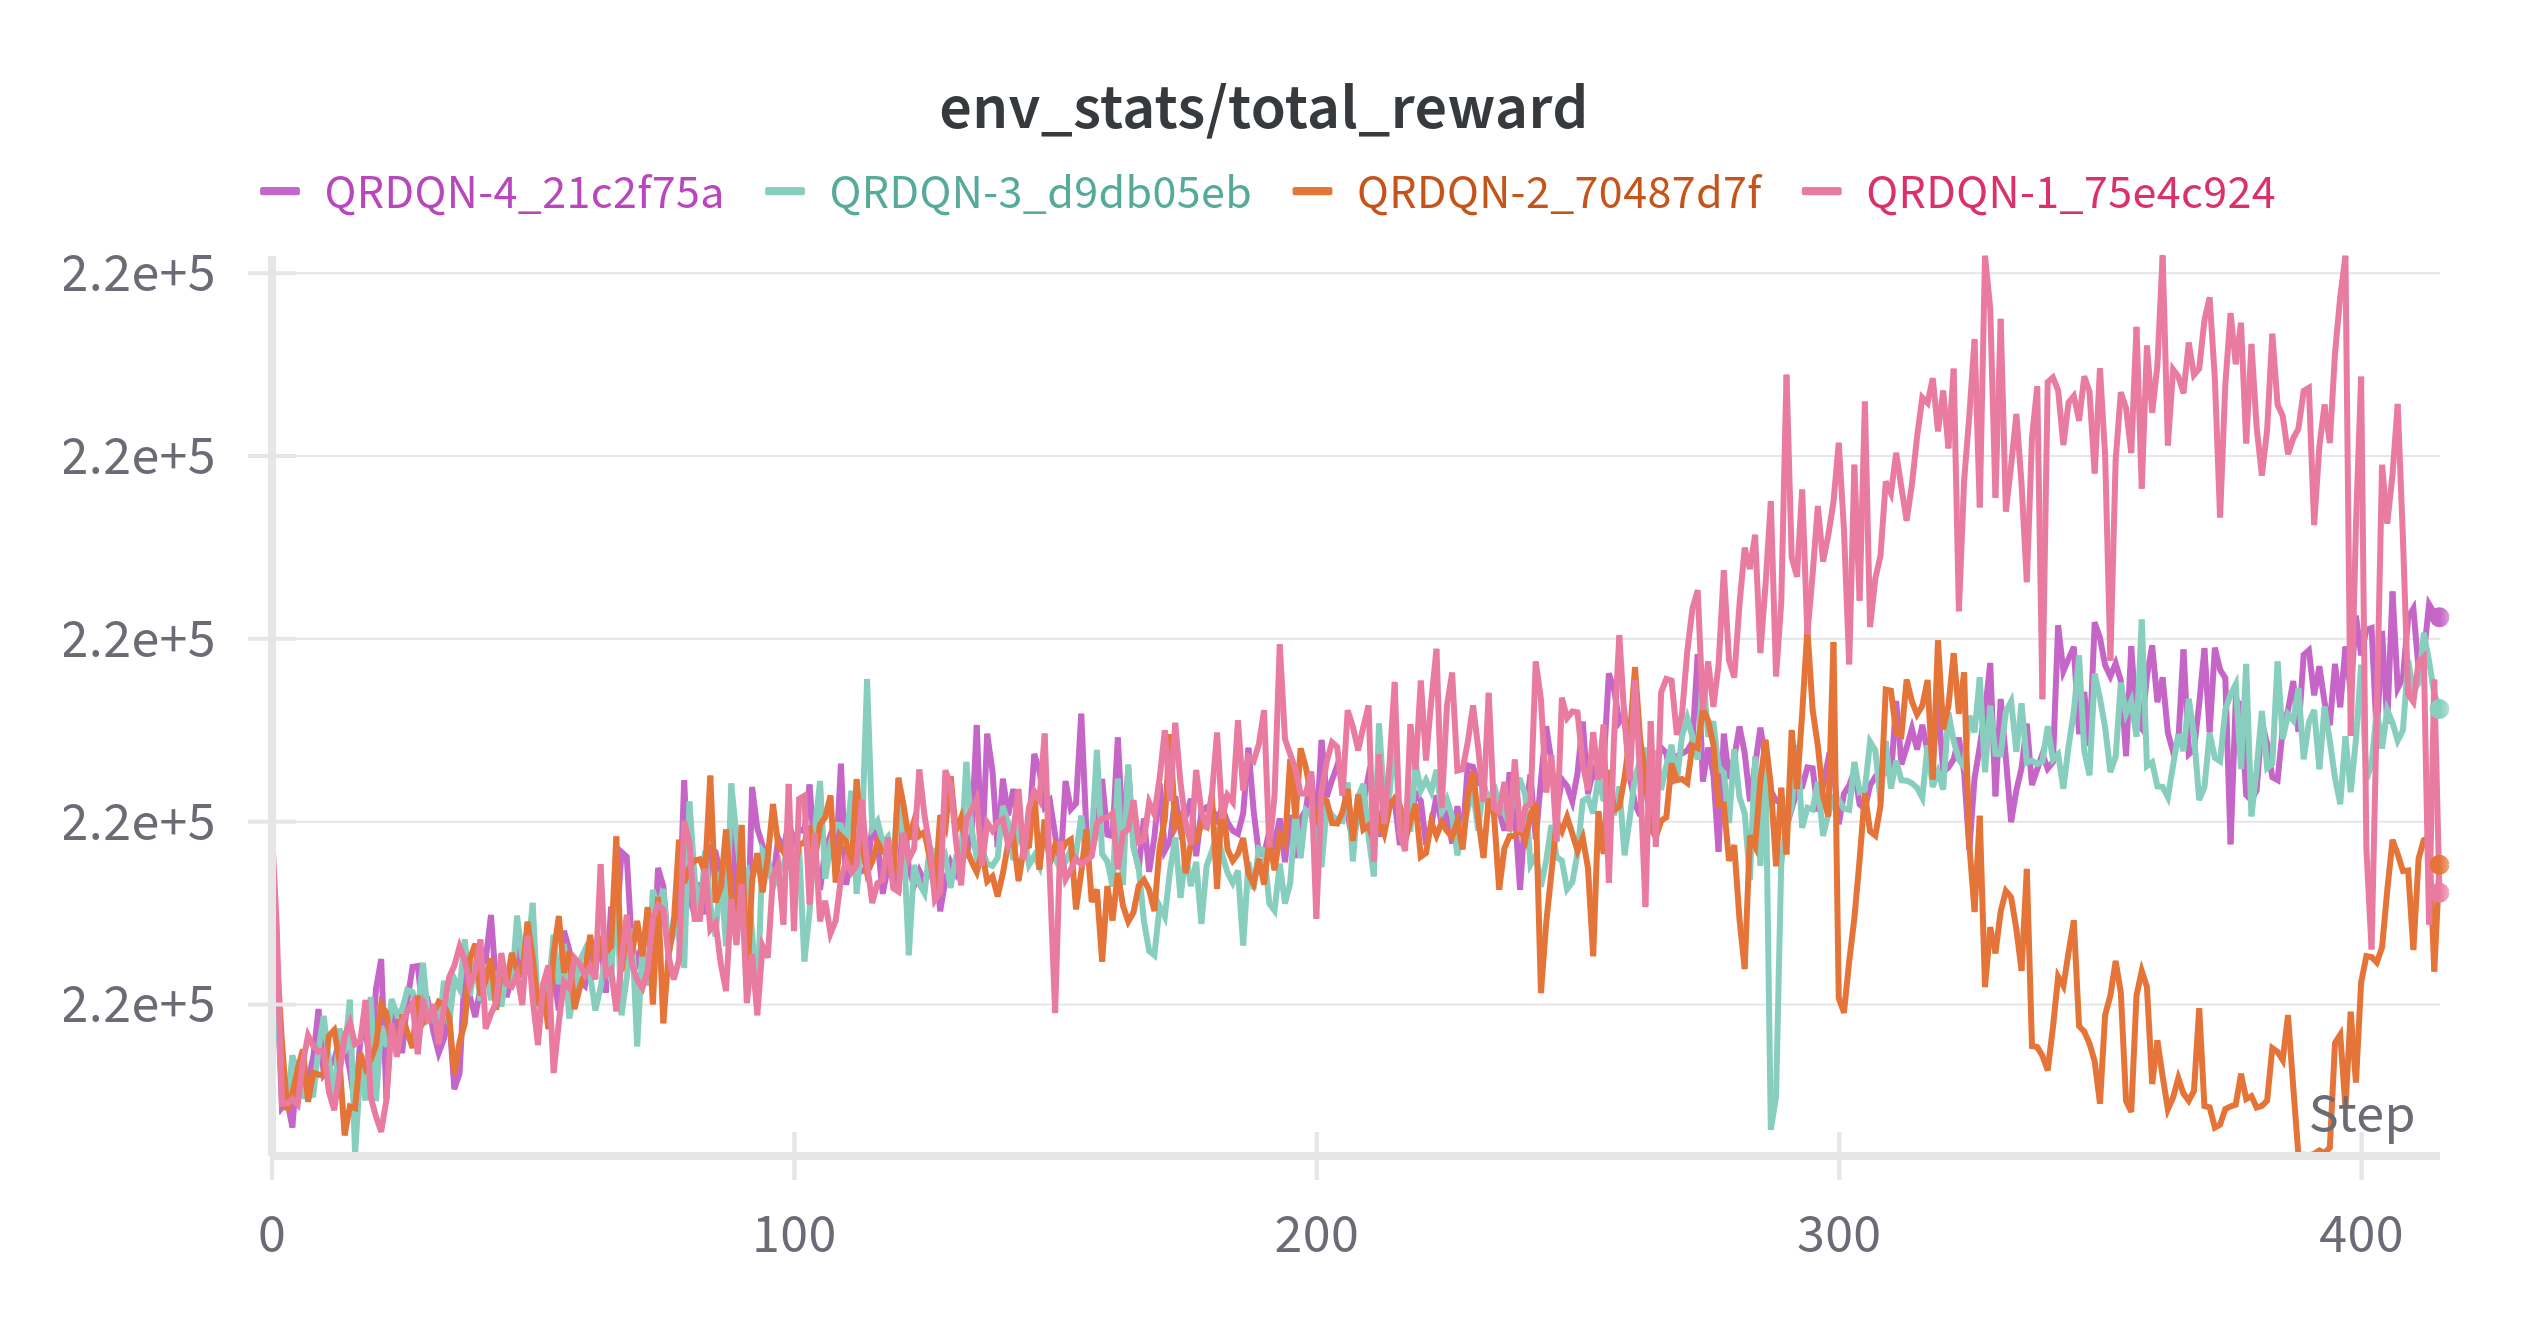
\includegraphics[width=0.8\textwidth]{figures/QRDQN_TotalReward.png}
    \caption{Total Reward of All QRDQN Agents}
    \label{fig:agent_eval_all_qrdqn}
\end{figure}

Compared to the DQN agents, the QR-DQN agents show a more promising performance in terms of total reward. The figure above shows the performance of all 4 QR-DQN agents of total\_reward against episode and shows that all 4 agents had a very similar but consistent growth in performance. Between episodes 0 and 200, all 4 agents had a similar amount of performance, but after episode 200, the agents started to diverge. QRDQN agent 3 and 4 had similar amounts of performance, where both agents had a very flat but consistently positive amount of growth. QRDQN agent 2 had a dramatic fall in performance from episode 270 to 370, but was able to swiftly recover and reach a peak performance at episode 400 but not enough data is available to determine if the agent would consistently kept this level of performance. QRDQN agent 1 spiked in performance and was able to maintain a high level of performance throughout the training, despite the sharp but short falls in performance every 50 episodes between episode 300 and 400. 

Despite the graph implying that QRDQN agent 1 is the best performing agent, only looking at the average total reward is not enough to come to this conclusion. Therefore, the graph below showing the average loss of each agent will be used to determine the best performing agent.

\begin{figure}[H]
    \centering
    \includegraphics[width=0.8\textwidth]{figures/QRDQN_Loss.png}
    \caption{Loss of All QRDQN Agents}
    \label{fig:agent_eval_all_qrdqn_loss}
\end{figure}

Figure \ref{fig:agent_eval_all_qrdqn_loss} showing the training loss of each agent shows that all 4 agents showed consistently low loss values with QRDQN agent 1 and 4 having large spikes of loss values of 8 and above. However, all agents had consistently low loss values with consistent random spikes, which further suggests that the best performing agent is QRDQN agent 1.

\subsection{PPO}

The training script used to train all 4 agents can be found within the research paper's GitHub repository under ``run\_baseline\_PPO.py''. A total of 14 parallel instances of the environment was trained at the same time to train for 1,905 episodes total, where each episode is 1,500 steps long. This totals up to 40,005,000 steps in total. The performance of the 4 agents can be seen in the graph below. 

\begin{figure}[H]
    \centering
    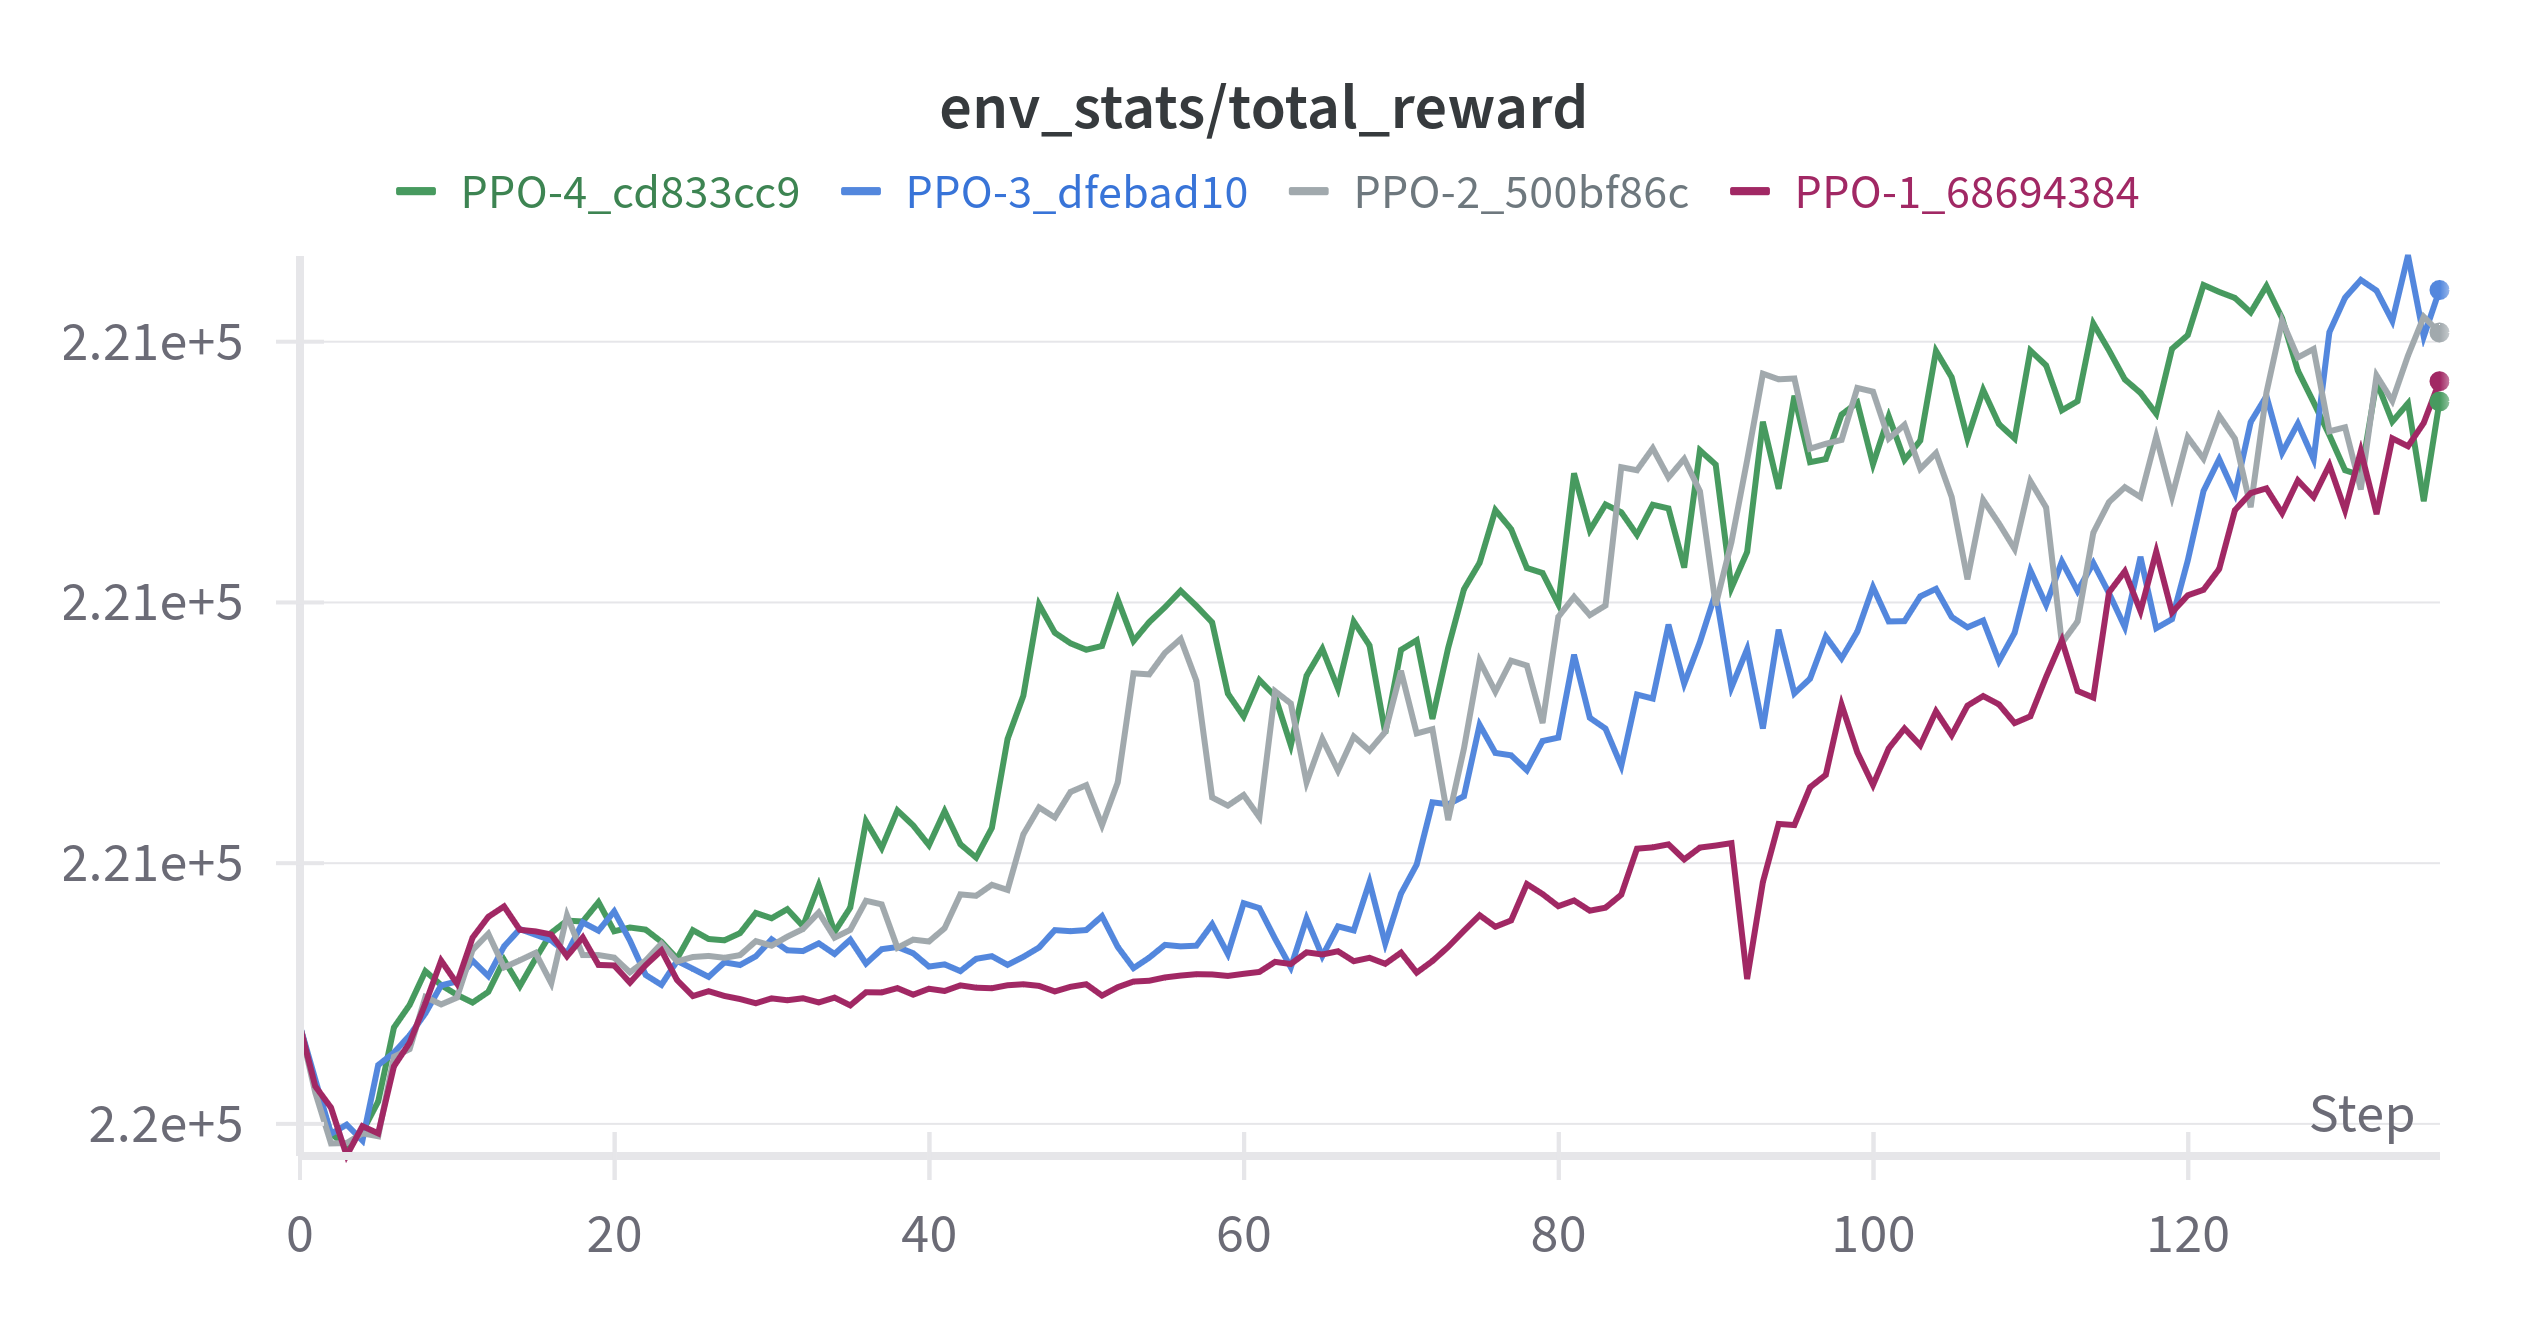
\includegraphics[width=0.8\textwidth]{figures/PPO_TotalReward.png}
    \caption{Total Reward of All PPO Agents}
    \label{fig:agent_eval_all_ppo}
\end{figure}

Looking at the performance of all 4 PPO agents, all the agents showed very strong signs of learning the environment and reaching the optimal policy. All agents maintained a gradual and strong growth in performance throughout training and all agents did not have any drops or sharp falls in total reward. Deciding the best performing agent among the 4 is difficult because all agents have very similar positive trajectories in performance. However, figure \ref{fig:agent_eval_all_ppo_loss}, below, showing the average loss of each agent will be used to find more information on the best performing agent.

\begin{figure}[H]
    \centering
    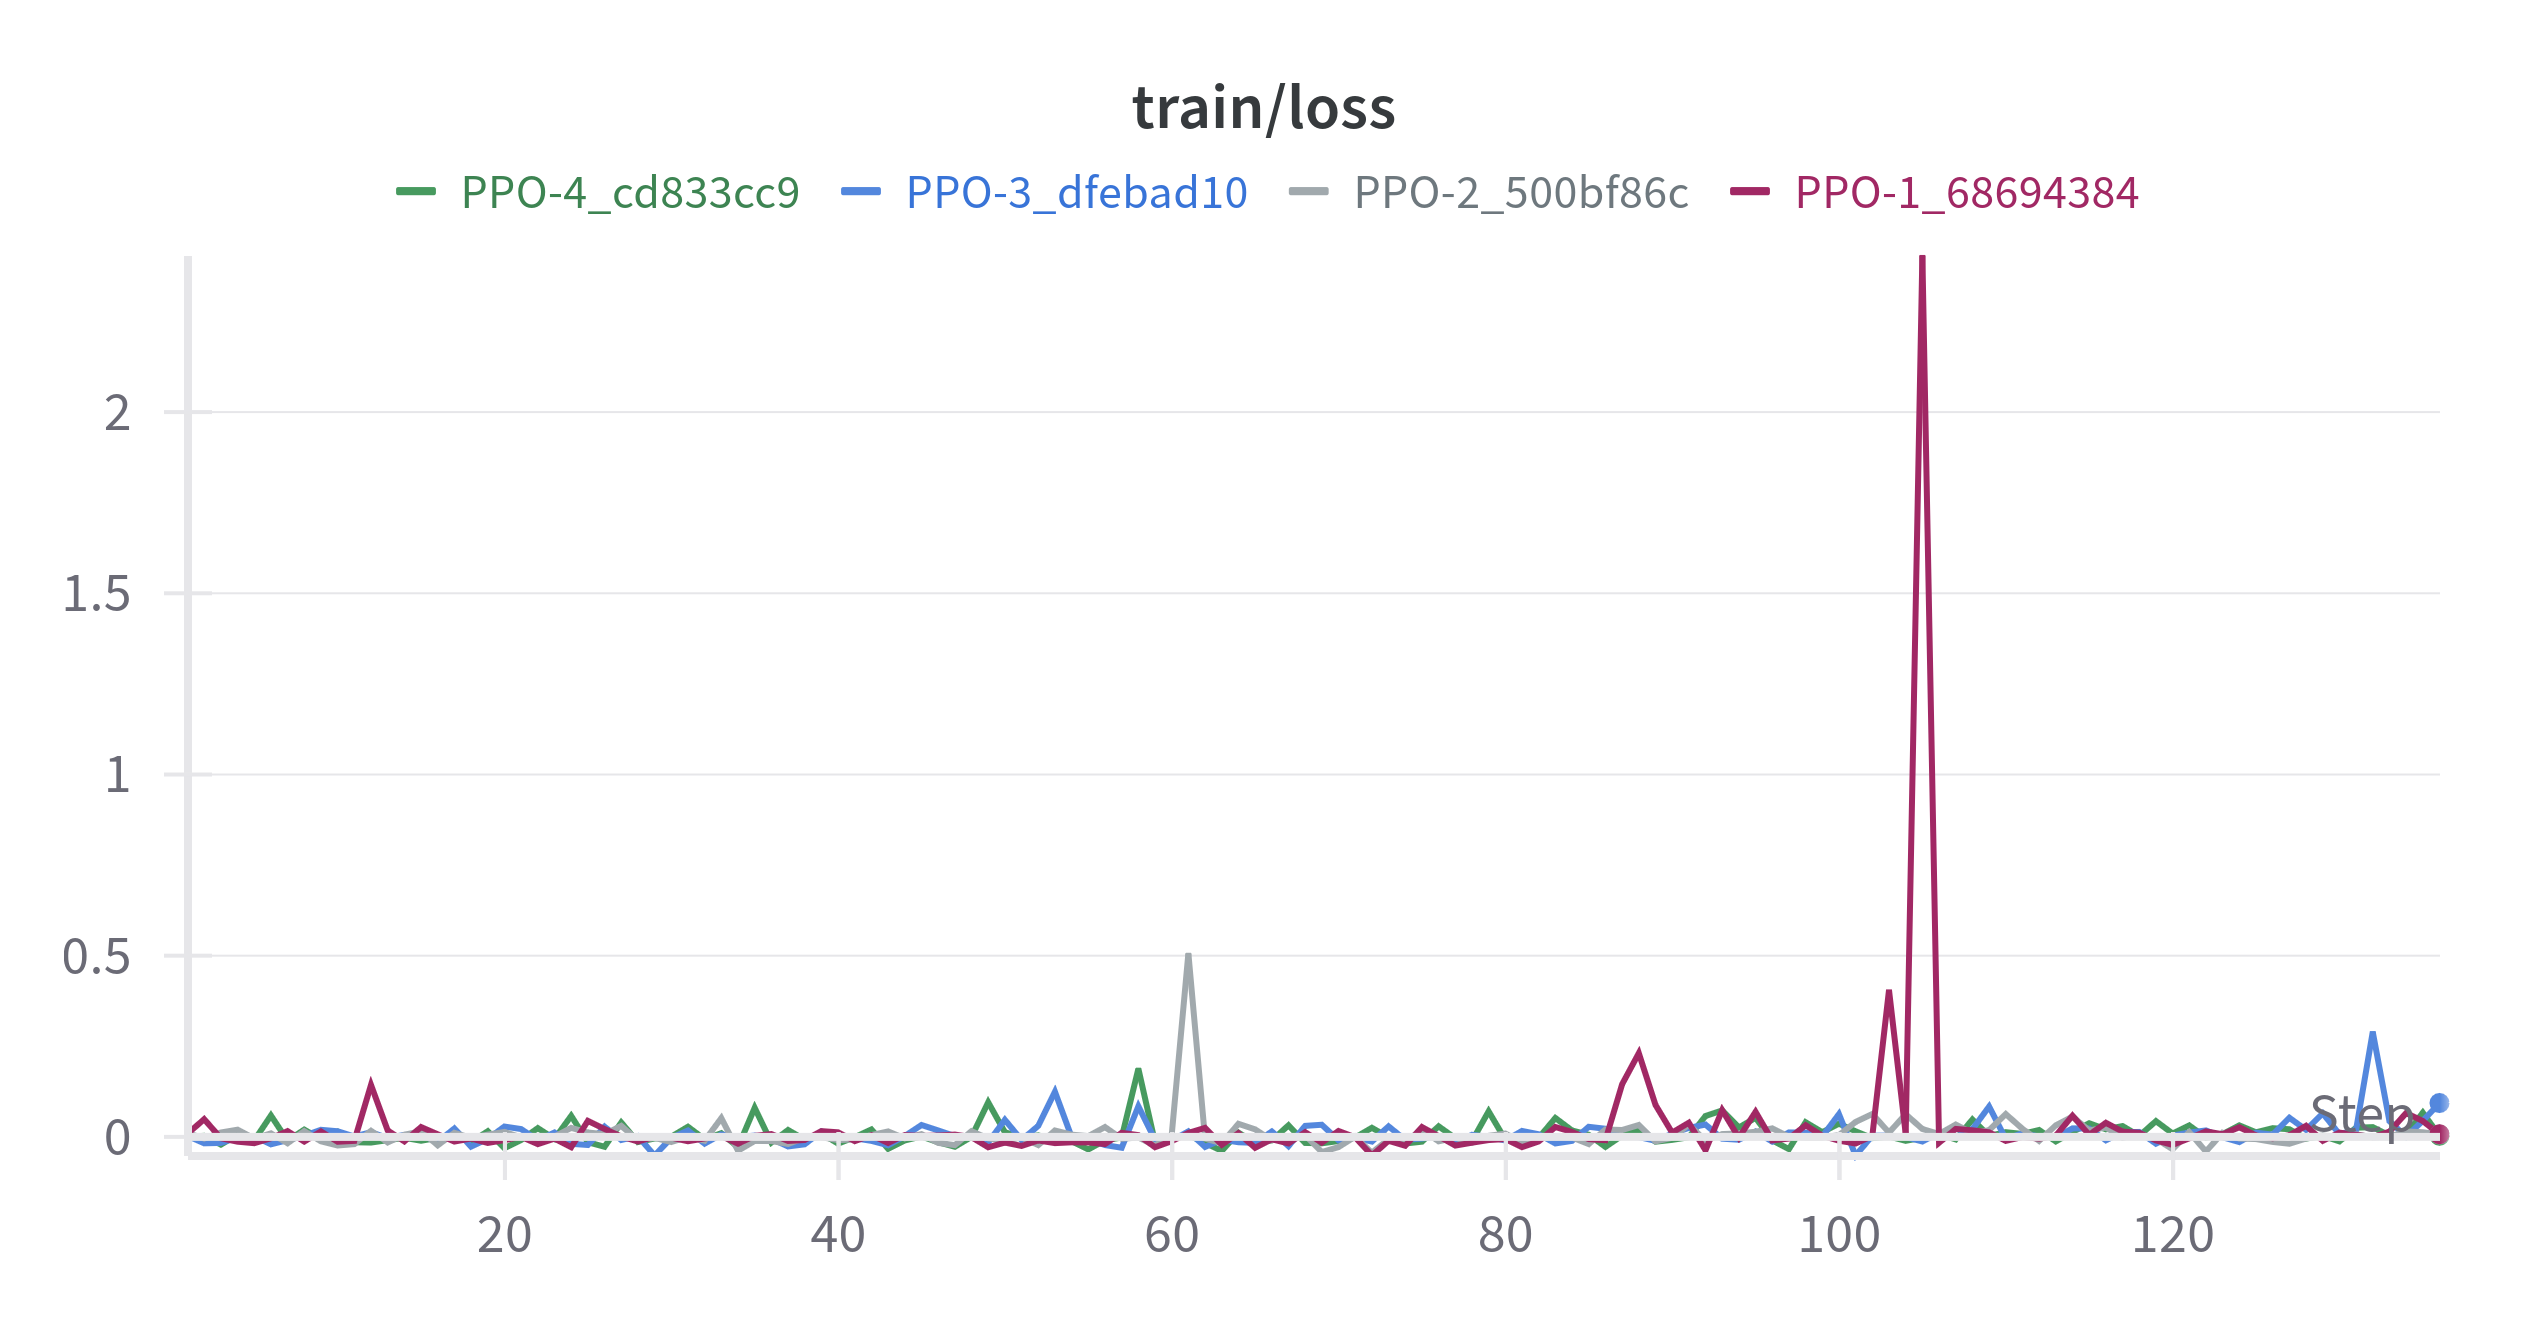
\includegraphics[width=0.8\textwidth]{figures/PPO_loss.png}
    \caption{Loss of All PPO Agents}
    \label{fig:agent_eval_all_ppo_loss}
\end{figure}

The figure above shows the training loss of each agent and shows that all 4 agents had consistently low loss values throughout the training with the exception of PPO agent 1, which had a large spike in loss at episode 100. Despite the spike in loss, the agent was able to recover and maintain a low loss value. However, the graph does not provide enough information to conclude the best performing agent, only that agent 1 experienced a large unexplanable spike in expected to experienced outcome. 

\begin{figure}[H]
    \centering
    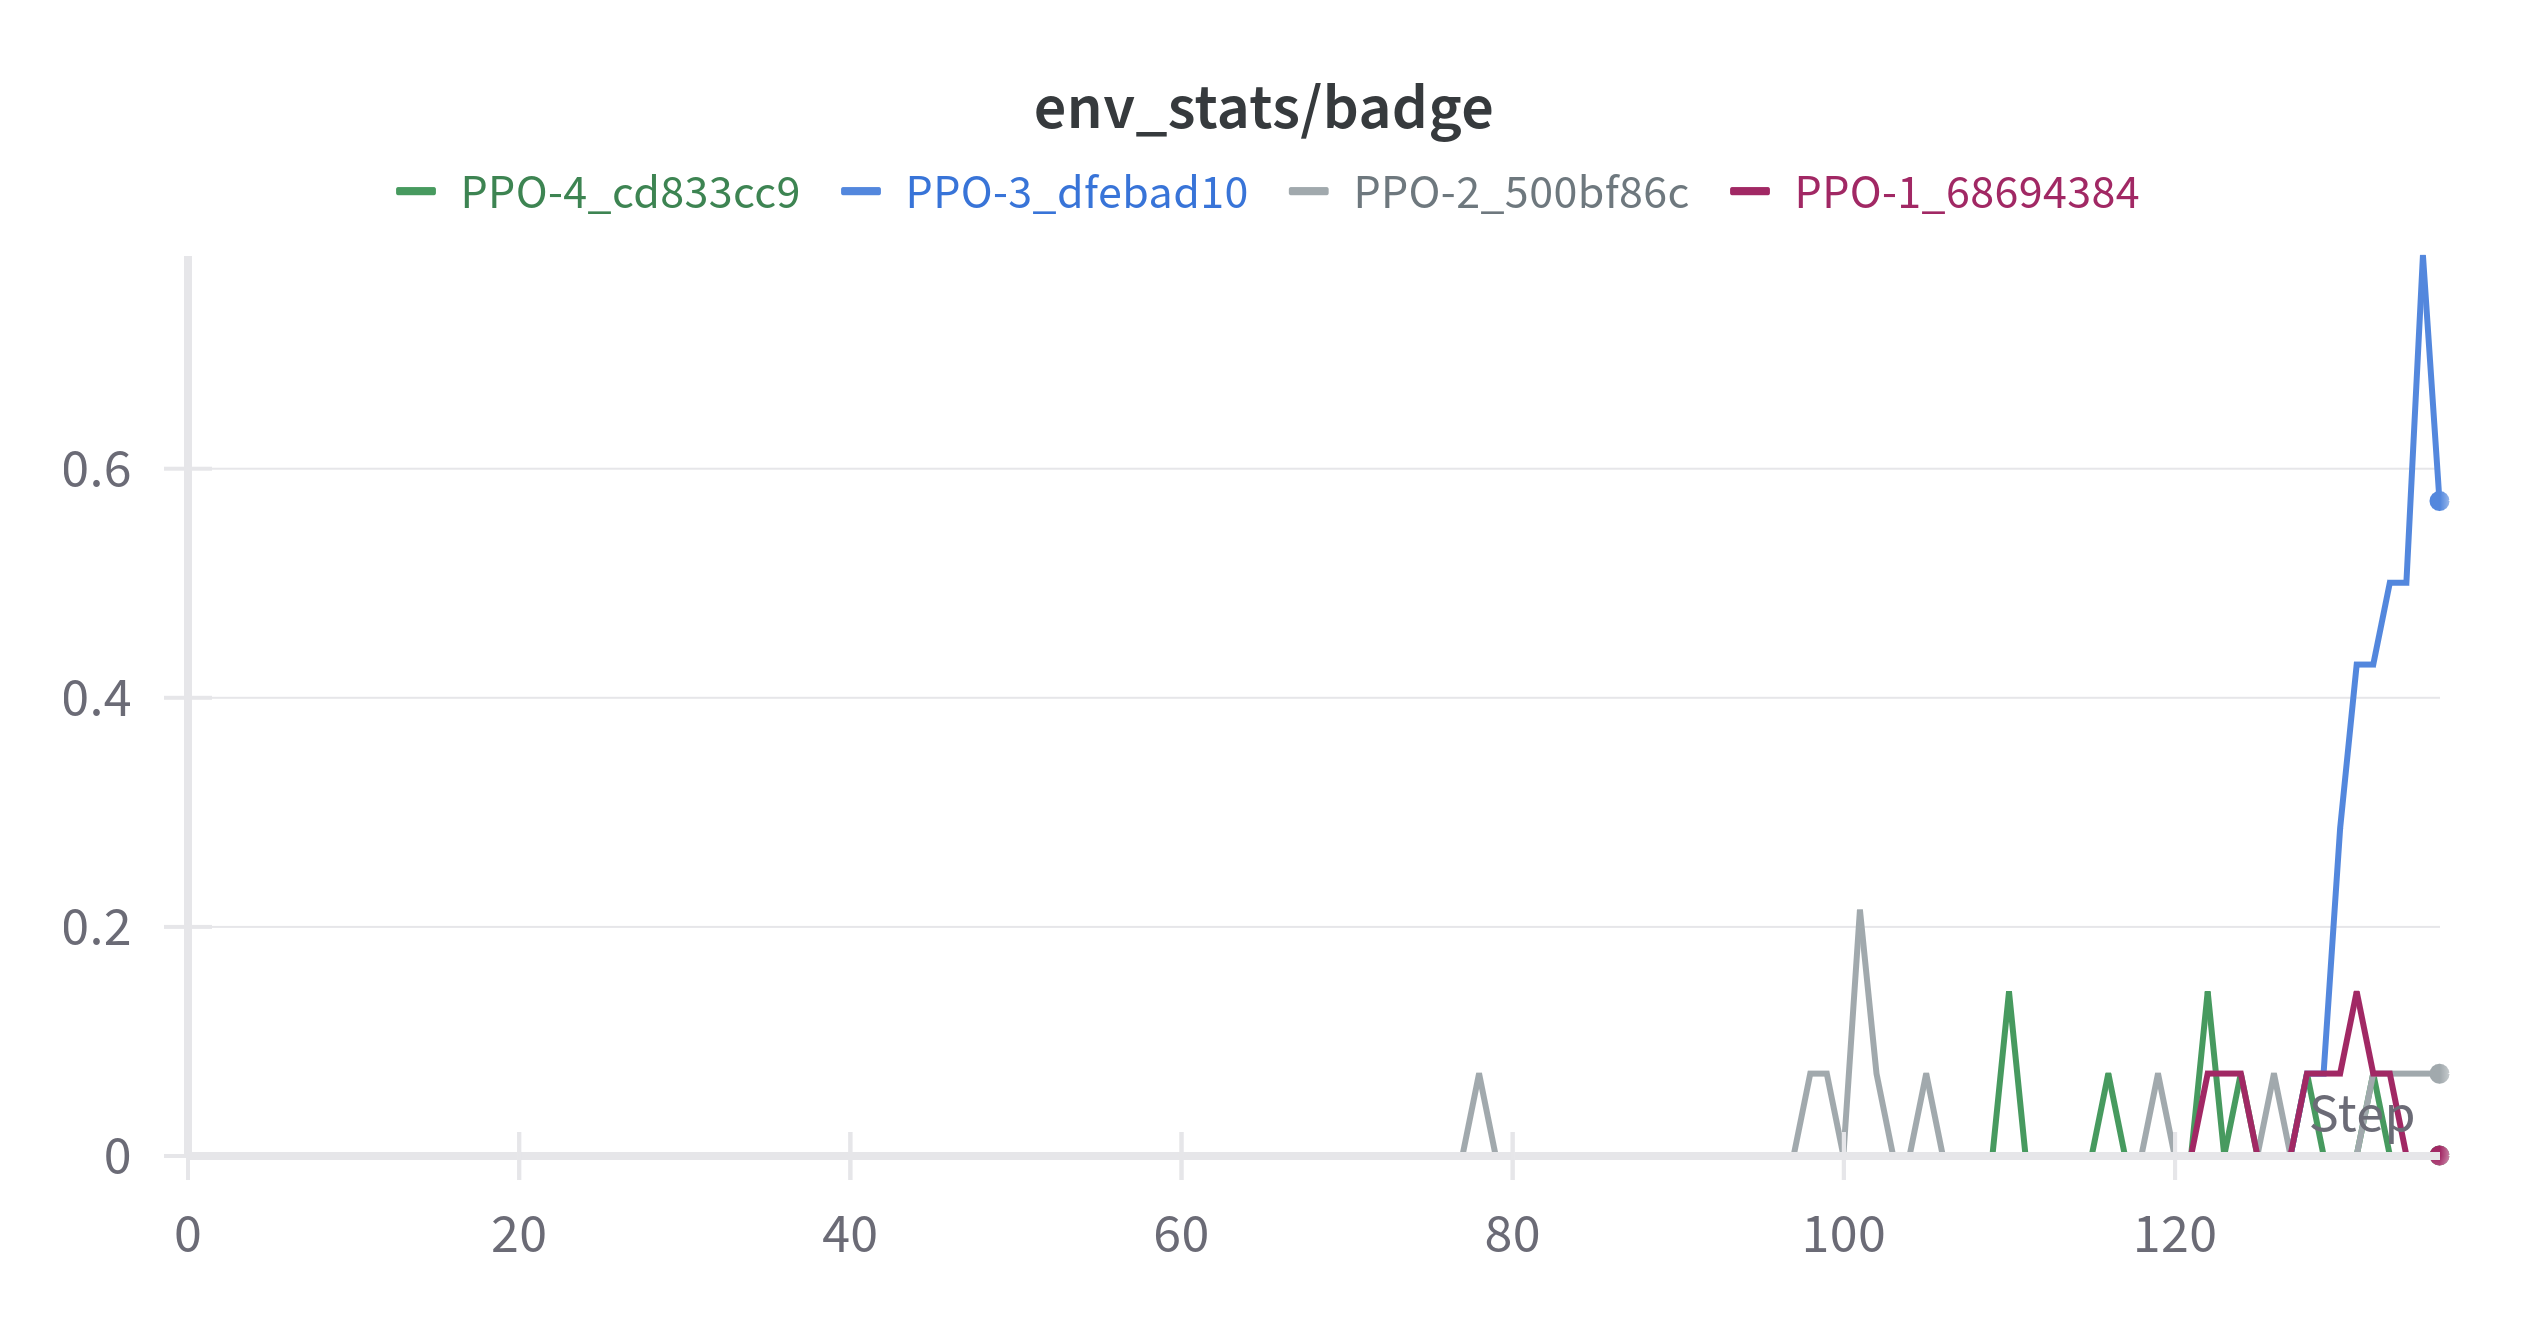
\includegraphics[width=0.8\textwidth]{figures/PPO_Badge.png}
    \caption{Badge Count of All PPO Agents}
    \label{fig:agent_eval_all_ppo_badge}
\end{figure}

To come to a conclusion as to which PPO agent is the best performing agent, figure \ref{fig:agent_eval_all_ppo_badge} showing the badge count of each agent will be used to determine which agent was able to complete the objective of this research the best by collecting the first gym badge the most consistently. The graph shows that all 4 agents were able to explore the environment enough to collect the first badge, however, PPO agent 2 was the agent to collect the first badge the earliest during training at episode 76. This is interesting as around the same episode, PPO agent 4 had a higher total\_reward than PPO agent 2. This suggests that the environment was explored differently by each agent and that the environment's reward function was not able to effectively guide the agent to reach the goal of collecting the first gym badge. Another interesting piece of information the graph confirms, is that agent 1 is the worst performing agent, as it was the second slowest agent to have one of the 10 instances collect the first gym, but also the agent with the least amount of consistency of instance of agents collecting the first gym badge. 

The most striking piece of information from the graph shows that agent 3 was the last to collect the first gym badge, but was the agent with the most consistent amount of instances to collect the first gym badge. With a peak of 80\% of the instances collecting the first gym badge by the end of training. This confirms that agent 3 is the best performing agent out of the 4 PPO agents.

\subsection{Algorithm Comparison}

The best performing agent from each algorithm will be compared to each other to determine which agent was able to balance out battling and navigation the best. The best performing agent from each algorithm was DQN agent 3, QR-DQN agent 1 and PPO agent 3. The performance of each agent will be compared through the use of comparing the total reward, loss, and badge count of each agent to determine their potential to complete the entire environment and how well they are able to achieve the objectives of this research within the training time frame of 40 million steps. 

One issue that arose while comparing the agents was that the agents were trained for different number of total episodes. Despite the total amount of timesteps being consistent betwewen all trained agents, the total amount of episodes was different because each algorithm had inconsistent number of instances of the environment being trained at the same time. This is because each algorithm took different amounts of RAM to train. Therefore, the graphs below will show the total timesteps taken on the x-axis instead of the total episodes. Next time, the number of environment instances and episodes will be kept consistent for further fairer testing. 

\begin{figure}[H]
    \centering
    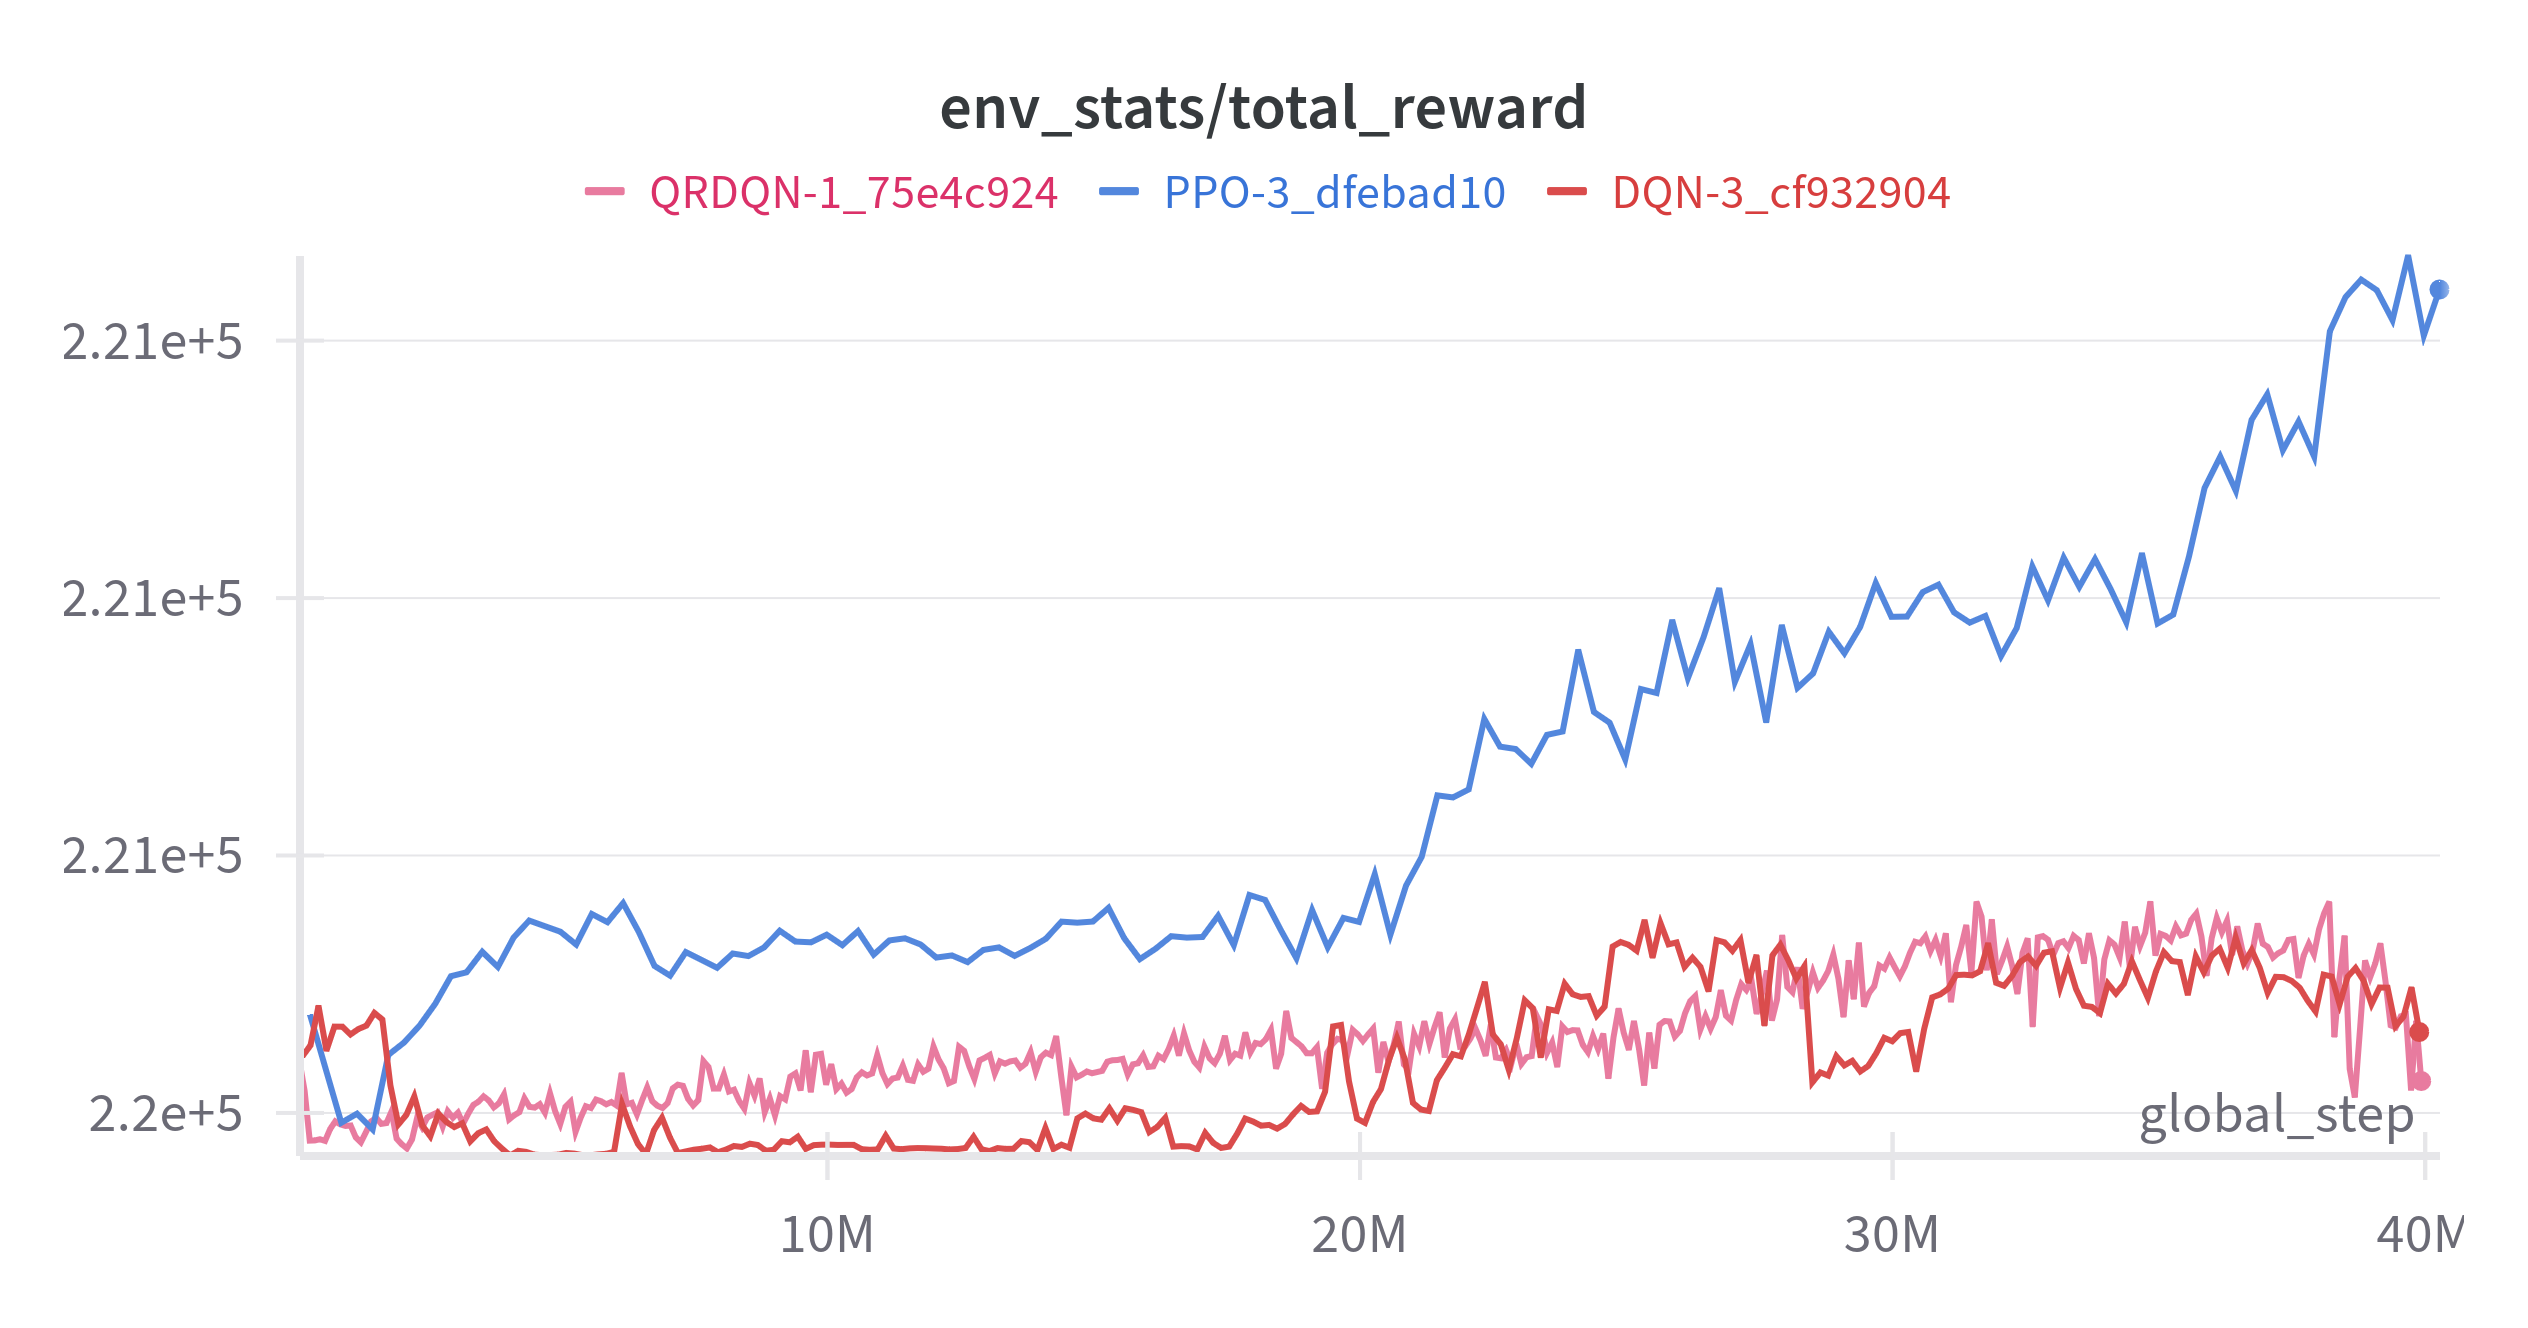
\includegraphics[width=0.8\textwidth]{figures/all_step_total_reward.png}
    \caption{}
    \label{fig:agent_eval_all_reward}
\end{figure}

Figure \ref{fig:agent_eval_all_reward} shows the total\_reward against total timesteps shows very evidently that PPO out performed DQN and QRDQN since the start. PPO was able to reach a higher amount of total reward within the first million timesteps compared to DQN and QRDQN. However, all 3 agents had similar rates of growth between 1 million and 20 million timesteps, which is suggested by the slopes of the agents being very similar. PPO showed a large increase in performance at around 20 million timesteps, which suggests that the agent was able to surpass a region of the environment which allowed for more reward to be gained. DQN and QRDQN comparitively did not show any signs of improvement in performance, which suggests that the agents were not able to reach the same region of the environment that PPO was able to reach. This is evident on figure \ref{fig:agent_eval_all_badge} below, showing the number of badges collected by each agent.

\begin{figure}[H]
    \centering
    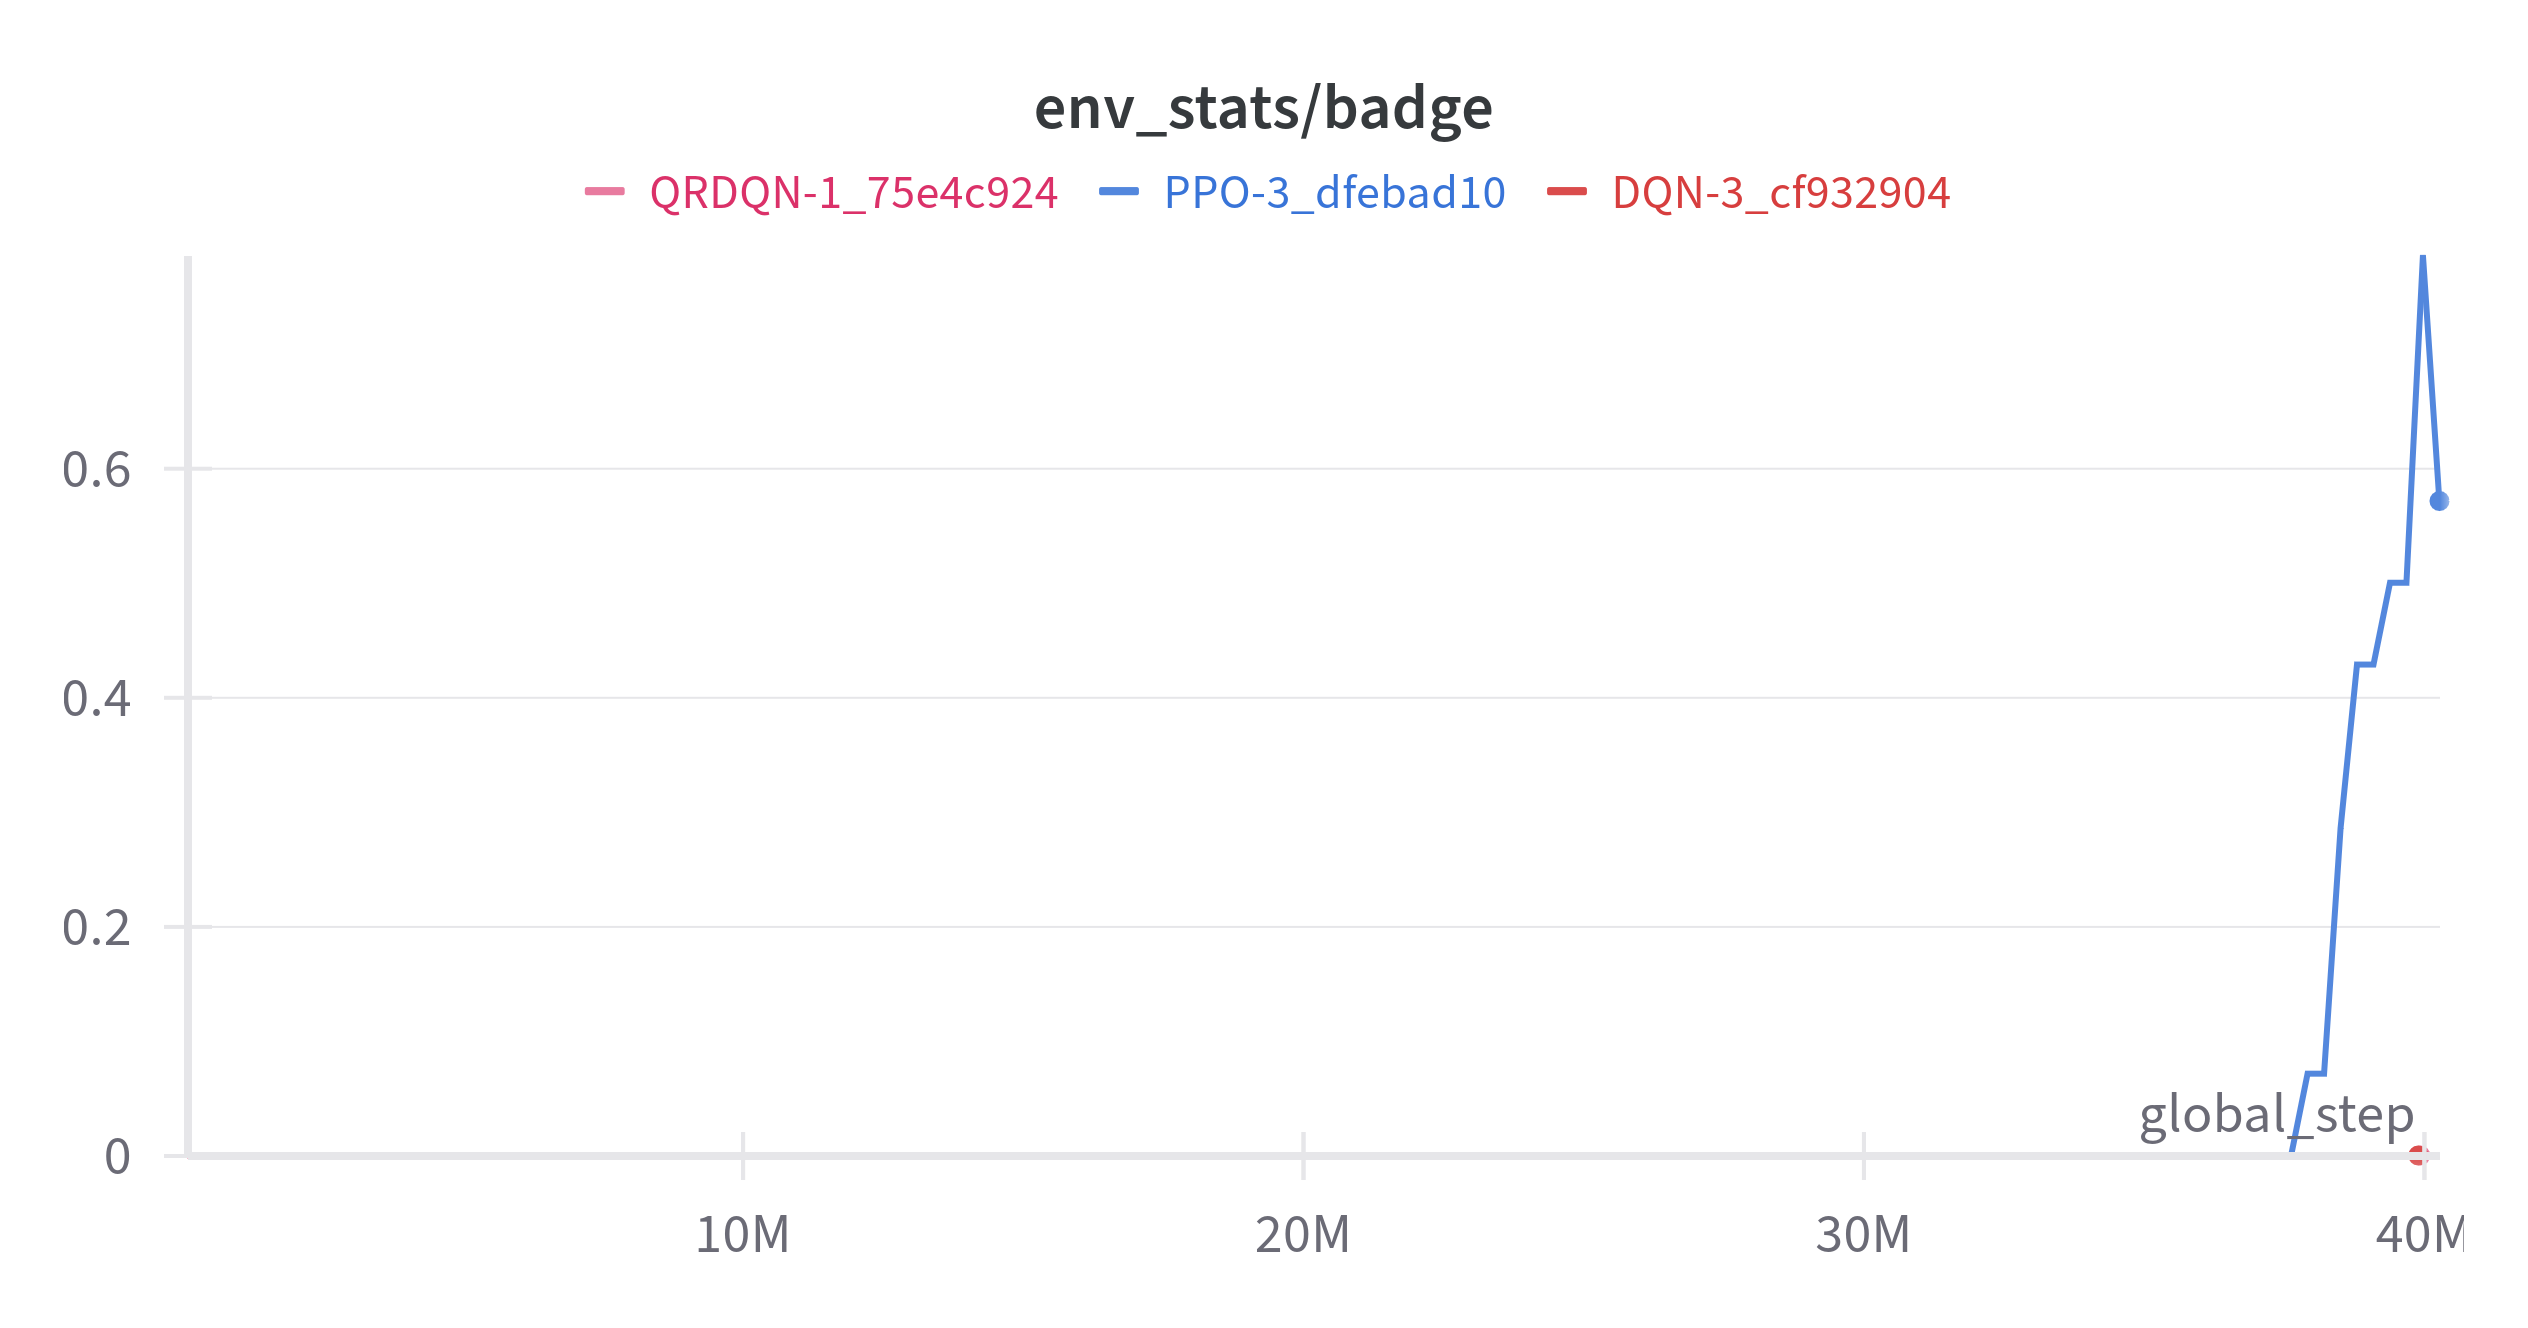
\includegraphics[width=0.8\textwidth]{figures/all_step_badge.png}
    \caption{}
    \label{fig:agent_eval_all_badge}
\end{figure}

This next graph shows the badge count of each agent against total timesteps. The graph shows that PPO was able to collect the first gym badge, where as DQN and QRDQN was never able to find the first gym badge. This suggests that PPO was able to explore the environment and overcome the challenges that DQN and QRDQN were not able to overcome, which is why PPO was the only agent able to collect the first gym badge. 

\begin{figure}[H]
    \centering
    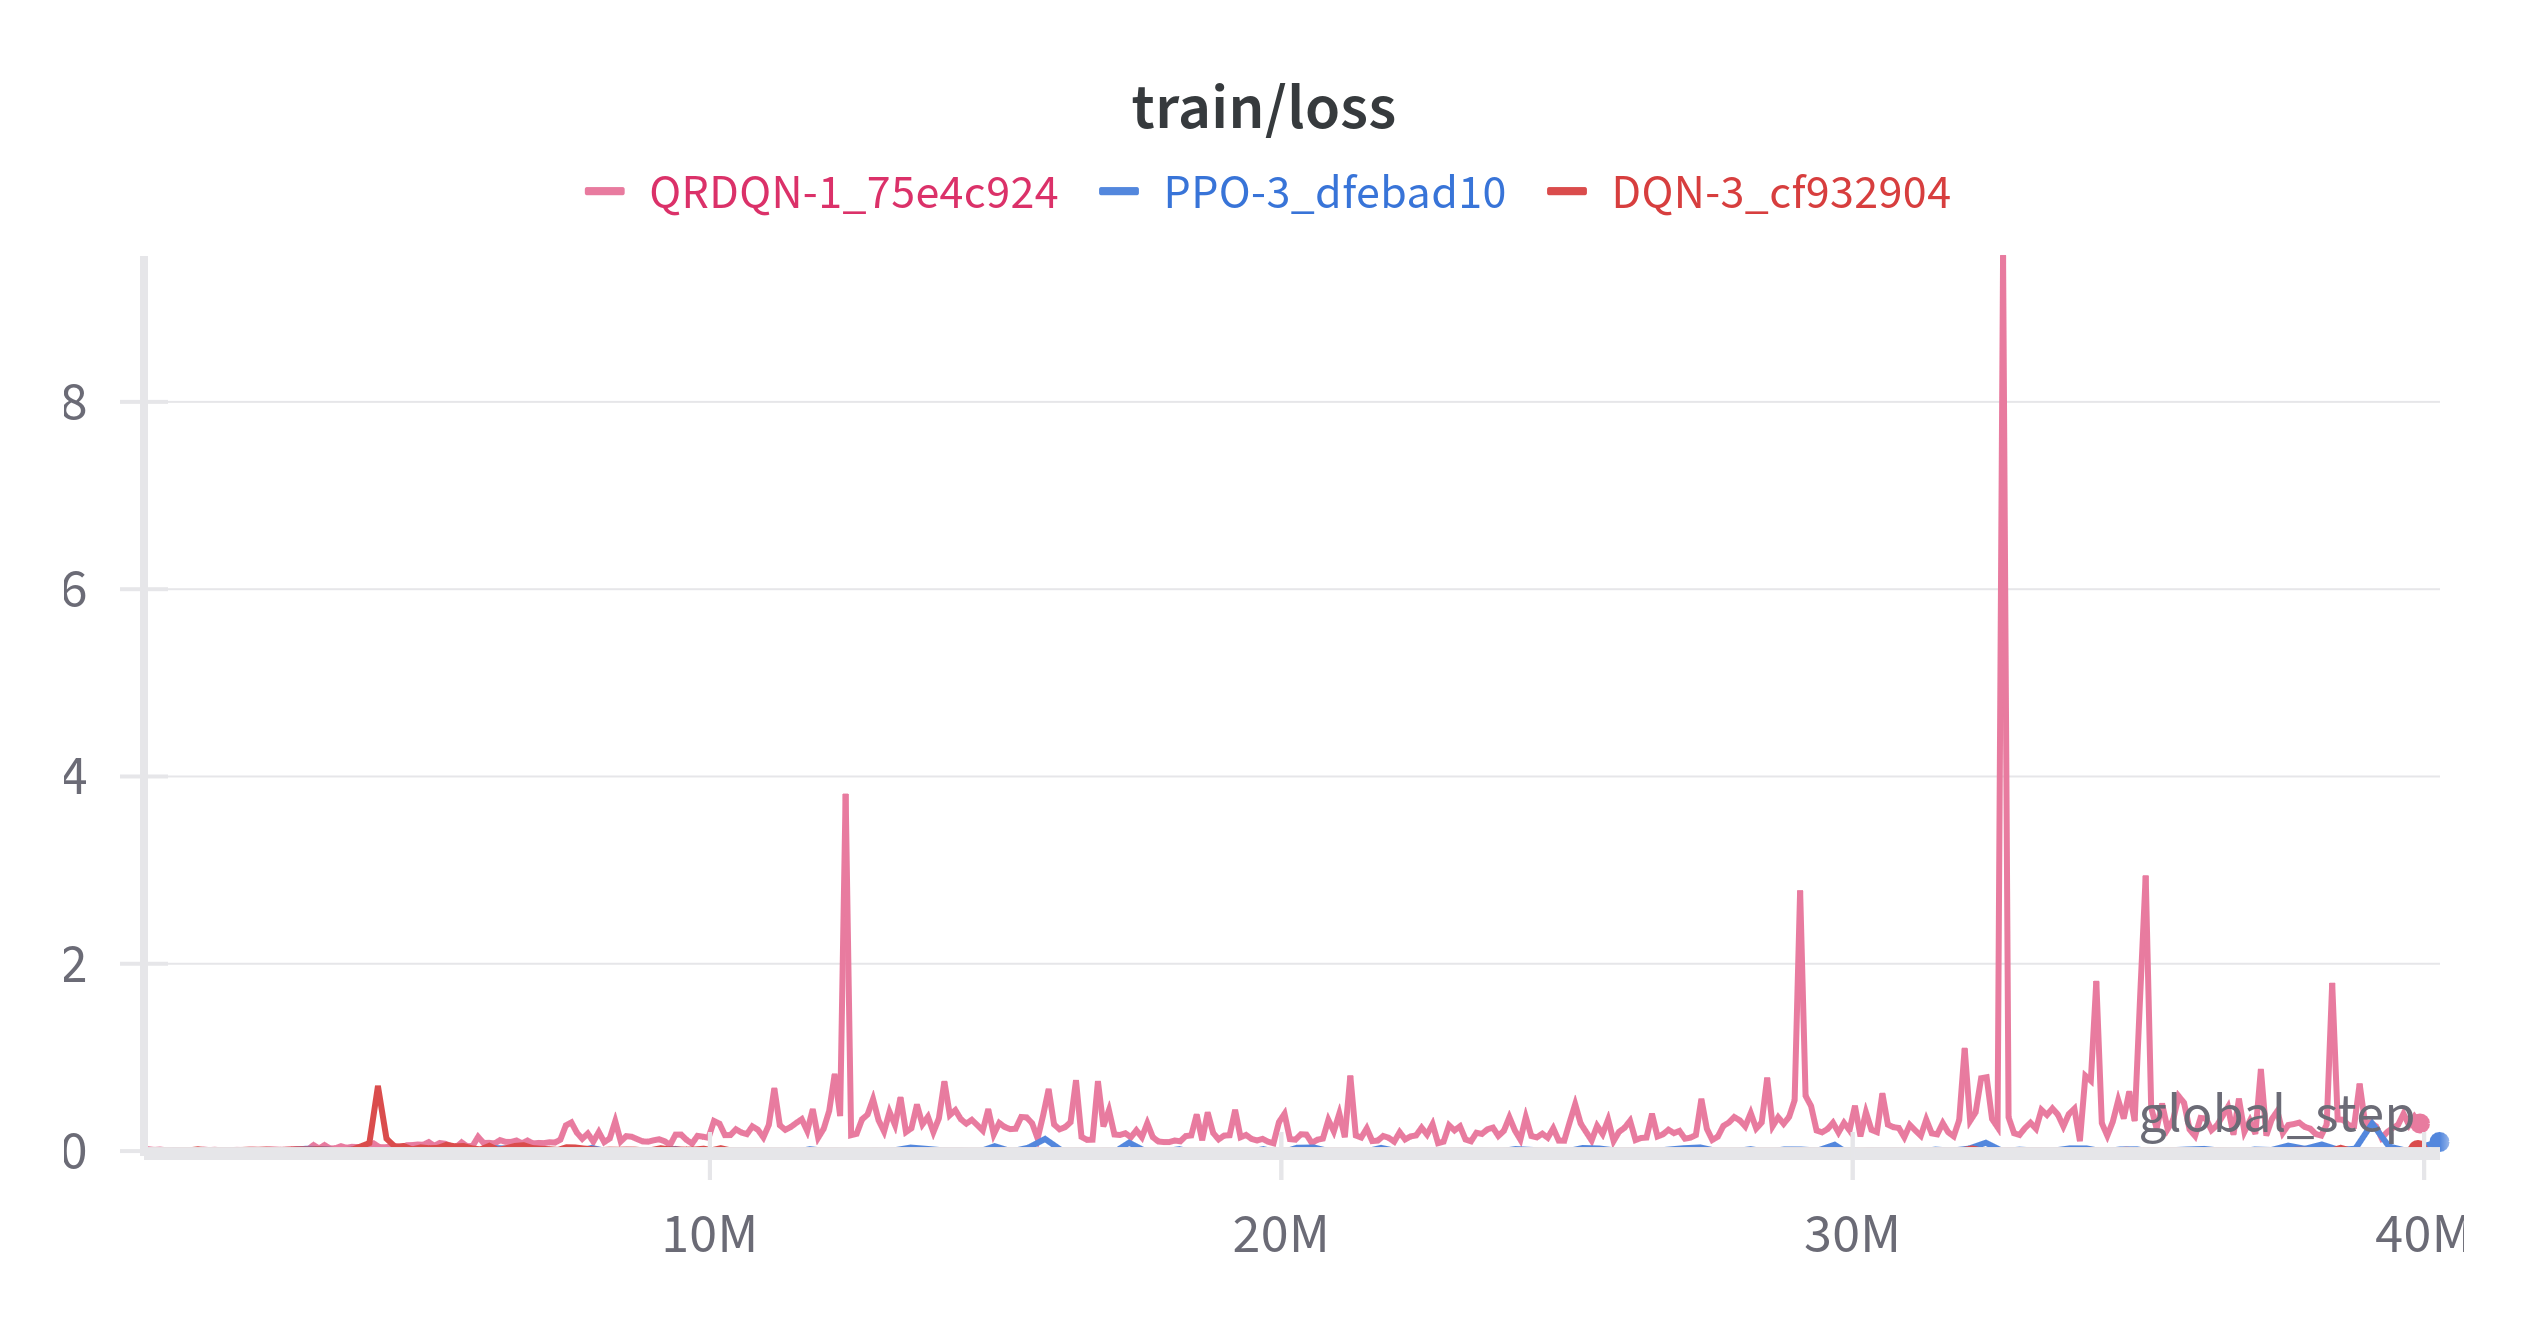
\includegraphics[width=0.8\textwidth]{figures/all_step_loss.png}
    \caption{}
    \label{fig:agent_eval_all_loss}
\end{figure}

Figure \ref{fig:agent_eval_all_loss} shows the loss of each agent against total timesteps. The graph very evidently highlights the turbulent nature of QRDQN training, as the agent had countless spikes of differing sizes. Where as DQN and PPO had very consistent low loss values throughout the training. This suggests that QRDQN had a very inconsistent training process and was not able to effectively learn what to expect within the environment compared to the actual outcome of the environment. It can be argued that the inconsistent training process is due to the low amount of reward achieved by QRDQN, which suggests that it was consistently exploring. However, the DQN agent had very similar levels of total reward to QRDQN and had a very consistent and low loss value while training. 

\subsection{Algorithm Comparison Conclusion}

In conclusion, it is evident that the PPO agent was the best performing agent out of the 3 agents. This is evident by the agents higher total reward, the only algorithm able to collect the first gym badge and the consistent low loss value throughout training. This suggests that value-based policies such as DQN and QRDQN are not as effective as policy-based policies such as PPO when training agents to explore and exploit the environment. However, it is difficult to find further research that agree with this conclusion, as there is a lack of benchmarks for multi-objective RL in the field. Moreover, there is a lack of popular well-known multi-objective RL environments that can be used to benchmark different algorithms unlike single objective RL. Despite the lack of benchmarks and research, Jett Wang's work using PPO to train agents to compete at high levels of pokemon battling suggests that PPO is a good algorithm to use for complex environments \cite{wang2020playing}. This is backed up by fact that Jett Wang's work was able to achieve far higher results than other works that focus on creating agents to do pokemon battling, while training the agent in a far more complicated environment. 

The other work to compare my findings to would be Flaherty, Jimenez and Abbasi's work in which they did train agents to complete pokemon red. However, their work compared DQN and A2C, where they found that A2C outperformed DQN due to A2C's greater timestep efficiency \cite{flaherty2021playing}. This would make for a great comparison between PPO and A2C because A2C uses both value and policy-based methods to train agents. This was one of the reasons why I initally chose to compare A2C as well to determine if I could reproduce similar results and if PPO was even more efficient than A2C. However, due to the lack of time and resources, I was not able to get A2C to work within the environment. 

It is possible that the stochastic nature and massive search space of this environment made it difficult for value-based policies to learn the environment effectively. As it was infeasible to explore each and every possible state within the environment. On the other hand, the reward function was fine-tuned to the PPO agent, which could have been the reason for the PPO agent outperforming the other agents. The complexity of the environment and the stochastic nature of the environment made it very difficult to determine an effective reward function without training agents to estimate the effectiveness of the reward function. 

Despite the total reward performance of DQN and QRDQN being similar, the loss value of the DQN agent were better than QRDQN because of its stable performance throughout all 40 million timesteps. This suggests that DQN was able to learn the environment more effectively than QRDQN because of its ability to make consistent reward expectation throughout training.

\section{Conclusion}

Within this section, the research project will be concluded by summarizing and reflecting on what worked well within the project, the challenges that I faced during the project, any improvements I would make and the future work to extend this research prroject.

\subsection{What worked well?}

During the research project, there were many aspects that worked well and contributed to the success of the project. However, one of the most useful tools that was taught during my 2nd year of university was the use of git version control. Git allowed me to work on the project on multiple different machines and keep a history of any changes. This was especially important as the project requried a lot of trial and error to get the algorithms to work correctly. In addition, when running the experiment on my main desktop, I was unable to use the computer for anything else, therefore being able to work from a secondary device allowed me to make better use of the available time.  

Another really important skill that I was taught during my year long placement was how to use tensorboard and evaluate the effectiveness of the model and the performance of each trained agenet. Tensorboard logging all of the information of the agent as it trained made it easy to see the progress of the agent and to determine if the agent was learning or not, as well as creating graphs to visualize the data for the report. Moreover, knowing what values to expect when evaluating a model made coming to a final conclusion more straight forward.  

The use of the OpenAI gym environment and the stablebaselines library written in Python were also very useful for this research project. In my final year of univeristy, python was used very extensively for all of the modules that I took, therefore a lot of transferable skills were able to be applied to this research project. In addition, the OpenAI gym environment was very easy to use and the support with stablebaselines3's implementation of the algorithms used for the experiment meant that I was able to focus more on the individuals details of the environment and worry less about writing the algorithms from scratch. 

Something else that helped with the most time consuming aspect of the research project, which was training the agent, was to use my own hardware. I was able to use my main desktop to train the agent throughout the day and night, which meant that I had more control over the amount of time that the agent was training. This potentially avoided any issues with the agent not training or any downtimes with any alterantive services I would have used. In addition, it was also more cost effective in the long-term to use my own hardware.

\subsection{Challenges}

While conducting this research, a quite a few issues arose that made the project more difficult to complete but were still able to be solved. The largest issue and main objective of this research was to find the correct reward function so that it was feasible for the agent to reach the goal of the firsy gym in order to compare their performances. The reward function of the multi-objective environment was difficult to implement correctly by balancing battling and navigation. The correct values were eventually discovered after countless agents being trained and tested, all of which can be found in the evaluation section of the report. However, being able to train an agent once during the day and once during the night sped up this process. 

The difficulty of tuning the reward function was contributed by the inital reward function that was provided by the environment. The environment had very simple rewards that were not enough to train an agent to complete the first gym, it was deigned to constantly train a singular agent till it eventually reached the goal. For example, the reward to encourage battling was static and would stop increasing the amount of reward given to the agent after reaching a certain level, which would result in the agent stopping to battle after reaching a certain point in the game. Another example was the reward for navigation, which would give a reward for ever new screen. However, this could be exploited by the agent by navigating through menus and not actually moving the character in the game. Instead, reward would only be given when a new screen is experienced and coordinates are updated. 

In addition, finding the correct number of total timesteps for the experiment was also difficult because it needed the value function to be corrected before further experimentation on an appropriate number of timesteps could be conducted. Initally, a value of 20 million timesteps was chosen, but was later increased to 40 million to ensure that the agents had enough time to learn the environment and reach the first gym more consistently. However, it was a time consuming task and required trial and error and lots of training time.

Another challenge that was faced during the research project was getting the inital algorithm script to work correctly. There were multiple examples of the algorithms being implemented in the stablebaselines3 library working with gym environments, however, the environment for this research was a custom gym environment and had to support multiple agents training on multiple instances of the environment, which is an added challenge. 

\subsection{Improvements}

If the research experiment were to be redone or extended in the short-term, many inital decisions and implementations would be done differently after gaining more knowledge and experience completing the experiment. 

The first improvement would be to find a method to shorten the training time of the agent. The agent took 5-6 hours to train, which meant that any changes to the environment took a long time to test. One way in which this could be shortened is to create a hyper accurate representation of the environment in a smaller scale without the use of an emulation. This would allow for the agent to be trained in a smaller environment allowing for less RAM to be used to load the ROM. In addition, removing the dependency on the gameboy emulator would allow for the environment to be further sped up. 

Another way in which I would improve this project would be to make the algorithm comparison more fair. The algorithms were not hyperparameter-tuned, which meant that the results were not comparable when at their best performance. Hyperparameter tuning would take a long amount of time to conduct but if more time were available, it would be a great way to compare the algorithms at their best performance. On the other hand, and algorithms were not trained for the same amount of episodes, which is another way I the algorithms were not compared fairly. The algorithms were trained for the same amount of timesteps, but due to differenct numbers of instances of agents training on the environment, the number of episodes completed was different. This was highlighted in the Evaluation section.

\newpage

\section{Future Work}

One way in which this project can be extended is to go beyond completing the first gym and to complete the entire game as intended. However, as I mentioned before, this would require longer episode lengths as the game is expected to take a human 25 hours long to complete. The game is not intended to be played in a singular session but to be played over multiple sessions. Two ways in which this can be shortened down is through the use of save states at the end of each gym or by using offline learning. 

For this experiment, I only used online learning, where the dataset is generated by the agent as it plays the game. However, offline learning would involve using a dataset before interacting with the environment. This dataset is generated by a human or another trained policy playing the game. This would allow the agent to learn from previous experiences and shortened the total training time as it does not require to start from zero previous knowledge. In addition, this technique could be implemented by saving the dataset generated by the agent, which just completed a gym, to be fed into the next agent that is going to defeat the next gym. In turn, making each gym a checkpoint of knoweldge for the agent. 

Another way in which the project can be extended to complete the entire game, would be to implement a checkpoint system at the end of each gym. Therefore, each agent would be tasked with getting from their starting position to completinig the next gym. This would be implemented by saving the game state when a gym badge is collected and stopping the training. A new untrained agent would then be loaded to continue from that save state. The downside to this method would be that it requires the agent to learn from scratch each time and not be able to use knowledge gained from the previous gym, which would make the project more akin to multiple policies learning to play the game rather than a single policy. In addition, requiring each agent to learn from scratch would increase training time, as the navigation and battling difficulty within the game is designed to increase as the player progresses through the game.

One way in which I wish this project could be extended or improved upon, would be to rewrite the reward function to be more generalized and less curated to the specific environment. Due to the similar nature of each generation of pokémon games, for example pokémon red, blue, yellow, gold, silver, etc, the reward function and get observation function could be rewritten to allow for a trained model to be used on any of the pokémon games. This would be a great example of showing the effectiveneses of RL in transfer learning, where a model trained on one environment can be used on another with similar goals. However, the reward function and observation function are too specific to the environment and rely on RAM readings to collect key information about the game state. All of the necessary information is theoretically available on the screen, such as the health of the pokémon, the level of the pokémon, the level of the enemy pokémon, etc, therefore it would be possible to have an external program read the necessary screen information and feed it into the environment. This would allow the agent to be trained on any pokémon game, to be deployed on any pokémon game. Moreover, this could be applied to all similar turn-based role-playing games. 
\section{Ethical Consideration}

When conducting research in any field, taking the ethical and legal considerations of the work conducted is as integral to the research conducted. Through out the work conducted in this project, all legal and ethical considerations have been taken into account. This was ensured through the guidance of my supervisor and by following the BCS Code of Conduct. In addition, following the ethical guidance of the University of Surrey, the Self-Assessment for Goverance and Ethics (SAGE) was completed to ensure that the research conducted was ethical and legal, which can be found at Appendix %! APPEND SAGE FORM HERE

\subsection{Data Collection}

No data was collected in this project. The data that was used was the Pokémon Red ROM, which was used to create the environment for the reinforcement learning agent. The data was not used for any other purpose than to create the environment for the agent to learn from. Therefore, the only type of data used for this research was directly used for the environments and no personal data was used for this research.

\subsection{Data Storage}

The limited data that is used is stored within the environment and only processed for the purpose of training the agent. The data in question is also not directly remembered or stored within the agent, only an association of how to react to the data within the environment is stored. Furthermore, no data is stored outside of the environment. 

\subsection{Legal \& Ethical Considerations: Do Not Harm}

The development of AI and machine learning has always been a field that has been scrutinised for the potential harm that it can cause in the future with its development. However, for the purposes of this research, the development of the reinforcement learning agent is limited to the environment of Pokémon Red, which is a game and holds no real world implications and marketed towards children. Therefore, the development of the agent is not harmful to any individual or group of individuals. Moreover, the greater purpose of this research is to assist the field of multi-objective reinforcement learning by providing more data for benchmarking and comparison, which holds just as many positive implications as negative.

\subsection{Legal \& Ethical Considerations: Informed Consent}

No human participation or data were required for this research to be conducted. Therfore, there was no need for informed consent to be obtained. 

\subsection{Legal \& Ethical Considerations: Confidentiality of Data}

No private, personal or confidental data was used for the purpose of this research. The only issue regarding this is the confidentality of the Pokémon Red ROM, which is owned by Nintendo. However, the use of the ROM was for educational purposes and not for commercial gain.
\section{References}
\printbibliography

\end{document}
